\newif\ifpictures
\picturestrue

\newif\ifjournal
\journaltrue

\newif\ifArXiv
\ArXivfalse

\documentclass[12pt]{amsart}
\usepackage{amssymb,amsmath}
 \usepackage{amsopn}
 \usepackage{xspace}
  \usepackage{hyperref}
 \usepackage[dvips]{graphicx}
\usepackage[arrow,matrix,curve]{xy}
\usepackage {color, tikz}
\usepackage{wasysym}
\usepackage[ruled,vlined]{algorithm2e}
\usepackage{graphicx}
\usepackage{subcaption}
\usepackage{mwe}
\usepackage{diagbox}


\headheight=8pt
\topmargin=30pt 
\textheight=612pt     \textwidth=456pt
\oddsidemargin=6pt   \evensidemargin=6pt

\numberwithin{equation}{section}
\newtheorem{thm}{Theorem}
\newtheorem{prop}[thm]{Proposition}
\newtheorem{lemma}[thm]{Lemma}
\newtheorem{cor}[thm]{Corollary}
\newtheorem{conj}[thm]{Conjecture}
\newtheorem{remark}[thm]{Remark}

\setcounter{secnumdepth}{5}

\theoremstyle{definition}

\newtheorem{definition}[thm]{Definition}
\newtheorem{example}[thm]{Example}

\numberwithin{thm}{section}


\newcounter{FNC}[page]
\def\newfootnote#1{{\addtocounter{FNC}{2}$^\fnsymbol{FNC}$%
     \let\thefootnote\relax\footnotetext{$^\fnsymbol{FNC}$#1}}}


\newcommand{\C}{\mathbb{C}}
\newcommand{\N}{\mathbb{N}}
\newcommand{\Q}{\mathbb{Q}}
\newcommand{\R}{\mathbb{R}}
\newcommand{\E}{\mathbb{E}}
\newcommand{\F}{\mathbb{F}}
\newcommand{\B}{\mathbb{B}}
\renewcommand{\P}{\mathbb{P}}
\newcommand{\TP}{\mathbb{TP}}
\newcommand{\Z}{\mathbb{Z}}

\newcommand{\tri}{\triangle}
\newcommand{\lf}{\left}
\newcommand{\ri}{\right}
\newcommand{\ra}{\rightarrow}
\newcommand{\la}{\leftarrow} 
\newcommand{\Ra}{\Rightarrow}
\newcommand{\La}{\Leftarrow}
\newcommand{\Lera}{\Leftrightarrow}
\newcommand{\ovl}{\overline}
\newcommand{\wh}{\widehat}
\newcommand{\lan}{\langle}
\newcommand{\ran}{\rangle}

\newcommand\cA{{\ensuremath{\mathcal{A}}}\xspace}
\newcommand\cB{{\ensuremath{\mathcal{B}}}\xspace}
\newcommand\cC{{\ensuremath{\mathcal{C}}}\xspace}
\newcommand\cD{{\ensuremath{\mathcal{D}}}\xspace}
\newcommand\cE{{\ensuremath{\mathcal{E}}}\xspace}
\newcommand\cF{{\ensuremath{\mathcal{F}}}\xspace}
\newcommand\cG{{\ensuremath{\mathcal{G}}}\xspace}
\newcommand\cH{{\ensuremath{\mathcal{H}}}\xspace}
\newcommand\cI{{\ensuremath{\mathcal{I}}}\xspace}
\newcommand\cJ{{\ensuremath{\mathcal{J}}}\xspace}
\newcommand\cK{{\ensuremath{\mathcal{K}}}\xspace}
\newcommand\cL{{\ensuremath{\mathcal{L}}}\xspace}
\newcommand\cM{{\ensuremath{\mathcal{M}}}\xspace}
\newcommand\cN{{\ensuremath{\mathcal{N}}}\xspace}
\newcommand\cO{{\ensuremath{\mathcal{O}}}\xspace}
\newcommand\cP{{\ensuremath{\mathcal{P}}}\xspace}
\newcommand\cQ{{\ensuremath{\mathcal{Q}}}\xspace}
\newcommand\cR{{\ensuremath{\mathcal{R}}}\xspace}
\newcommand\cS{{\ensuremath{\mathcal{S}}}\xspace}
\newcommand\cT{{\ensuremath{\mathcal{T}}}\xspace}
\newcommand\cU{{\ensuremath{\mathcal{U}}}\xspace}
\newcommand\cV{{\ensuremath{\mathcal{V}}}\xspace}
\newcommand\cW{{\ensuremath{\mathcal{W}}}\xspace}
\newcommand\cX{{\ensuremath{\mathcal{X}}}\xspace}
\newcommand\cY{{\ensuremath{\mathcal{Y}}}\xspace}
\newcommand\cZ{{\ensuremath{\mathcal{Z}}}\xspace}

\newcommand{\eps}{\varepsilon}
\newcommand{\vphi}{\varphi}
\newcommand{\alp}{\alpha}
\newcommand{\lam}{\lambda}
\newcommand{\kro}{\delta}
\newcommand{\sig}{\sigma}
\newcommand{\Sig}{\Sigma}
\newcommand{\lap}{\Delta}
\newcommand{\Gam}{\Gamma}


\definecolor{DarkGreen}{rgb}{0,0.65,0}
\newcommand{\yixuan}[1]{{\color{orange} \sf $\clubsuit\clubsuit\clubsuit$ Yixuan: [#1]}}
\newcommand{\mareike}[1]{{\color{cyan} \sf $\clubsuit\clubsuit\clubsuit$ Mareike: [#1]}}
\newcommand{\assum}{{\color{red} \sf $(\clubsuit)$}}
\newcommand{\durch}[1]{\textcolor{red}{\sout{#1}}}


\newcommand{\struc}[1]{{\color{blue} #1}}
\newcommand{\alert}[1]{{\color{red} #1}}


\DeclareMathOperator{\sgn}{sgn}
\DeclareMathOperator{\conv}{conv}
\DeclareMathOperator{\supp}{supp}
\DeclareMathOperator{\tconv}{tconv}
\DeclareMathOperator{\dist}{dist}
\DeclareMathOperator{\lin}{lin}
\DeclareMathOperator{\trop}{trop}
\DeclareMathOperator{\aff}{aff}
\DeclareMathOperator{\LP}{LP}
\DeclareMathOperator{\Arg}{Arg}
\DeclareMathOperator{\Log}{Log}
\DeclareMathOperator{\New}{New}
\DeclareMathOperator{\tdeg}{tdeg}
\DeclareMathOperator{\vol}{vol}
\DeclareMathOperator{\re}{re}
\DeclareMathOperator{\im}{im} 
\DeclareMathOperator{\odd}{odd} 
\DeclareMathOperator{\even}{even} 
\DeclareMathOperator{\ord}{ord}
\DeclareMathOperator{\Circ}{Circ}

\DeclareMathOperator{\res}{res}
\DeclareMathOperator{\sign}{sign}
\DeclareMathOperator{\grad}{grad}
\DeclareMathOperator{\RE}{Re}
\DeclareMathOperator{\IM}{Im}
\DeclareMathOperator{\w}{\wedge}
\DeclareMathOperator{\val}{val}
\DeclareMathOperator{\Val}{Val}
\DeclareMathOperator{\coA}{\text{co}\cA}
\DeclareMathOperator{\coL}{\text{co}\cL}
\DeclareMathOperator{\eq}{eq}
\DeclareMathOperator{\app}{app}
\DeclareMathOperator{\Tr}{Tr}
\DeclareMathOperator{\ini}{in}
\DeclareMathOperator{\Ker}{Ker}
\DeclareMathOperator{\Mat}{Mat}
\DeclareMathOperator{\Int}{int}
\DeclareMathOperator{\SOS}{SOS}
\DeclareMathOperator{\prep}{Prep}
\DeclareMathOperator{\rank}{rank}

\DeclareMathOperator{\verti}{Vert}
\DeclareMathOperator{\coeffs}{coeffs}


\def\endexa{\hfill$\hexagon$}

\title{Honors Project}

\author{Yixuan Zhou} %\author{}

\address{8514 Villa La Jolla Drive \# 114, La Jolla, CA, 92037\medskip}
\email{yiz044@ucsd.edu}

% \address{9500 Gilmam Drive \# 0112, La Jolla, CA, 92093 \medskip}
% \email{mdressler@ucsd.edu}



%\subjclass[2010]{Primary: 14P10, 90C25; Secondary: 12D05, 52B20}
\keywords{some keywords go here}


\begin{document}
 

\begin{abstract}
Polynomial optimization is widely applicatible in solving both practical and theoretical computation problem. 
One particularly successful way to solve the polynomial optimization certifying the nonnegativity of a polynomial using 
the sum of squares (SOS) certificate. In this thesis, we study how different choices of 
the polynomial basis can affect the numerical stability of the linear system generated when using Semidefinite programming (SDP) to 
test SOS. We run numerical experiments comparing the performance of monomial basis and different types of 
orthogonal basis, and we discuss the different trade-offs between the choice two types of polynomial basis. 
\end{abstract}

\maketitle


\section{Introduction} 

\emph{Polynomial optimization problems} are ubiquitous in applied mathematics and engineering. 
For instance, Ahmadi and Majumdar \cite{ahmadi2015applications} suggested to use
polynomial optimization in the field of \emph{artificial intelligence} for solving
\emph{real-time decision problems}. 
In electric power system design, the \emph{optimal power flow problem}
can be reduced to a polynomial optimization problem as well, see \cite{josz:tel-01478431}.

In general, an \emph{optimization problem} takes the form 
\begin{equation}
     \label{eq:optimization problem}
     \begin{split}
          \min_{\mathbf{x}} \ f(\mathbf{x}) & \quad \textit{subject to } g_i(\mathbf{x}) \geq 0 \\
          & \quad \quad \quad \text{ \ \ \ \ \ \  } h_j(\mathbf{x}) = 0, 
     \end{split}
 \end{equation}
where $f, g_i, h_j$ are arbitrary functions of the variables $\mathbf{x} = (x_1, ..., x_n)$. 
The function $f$ is called the \emph{objective function}, and the functions $g_i, h_j$ are called the \emph{constraints}.
Hence, when solving an optimization problem, one tries to minimize the objective function subject to certain constraints.
There are several ways to address this problem, which are collected as \emph{nonlinear optimization methods}. 
Some famous optimization approaches are the \emph{gradient decent} and \emph{Newton's method}. 
Those optimization algorithms seek to exploit the properties of the objective function to find a
local minimizer $\mathbf{x}^*$ and hope (with justifications in special cases) that the function value at the minimizer is close
to the global minimum. Whereas polynomial optimization takes a different approach.

Polynomial optimization, as the name suggests, is the specific case when the functions $f, g_i, h_j$ in \eqref{eq:optimization problem} are polynomials.
In this thesis, we focus on unconstrained polynomial optimization, that is, the feasible domain is $\mathbb{R}^n$.
Then, instead of minimizing a polynomial, one can search for its maximal lower bound.
Hence, we can equivalently formulate the unconstrained problem as 
\begin{equation*}
     \max \ r \quad \textit{s.t. } f(\mathbf{x}) - r \geq 0 \quad \textit{for all } \mathbf{x} \in \mathbb{R}^n,
 \end{equation*}
where the objective function $f$ is a polynomial, and the lower bound $r$ is a real number. 

To solve this problem, we need to decide whether a given polynomial is \emph{nonnegative} (see Definition \ref{def:NGP}).
It turns out that this problem has been well studied in real algebraic geometry since the beginning of the 19th century. 
However, it turns out that deciding whether an arbitrary multivariate polynomial is nonnegative is,
in the language of computational complexity, \emph{co-NP-hard} (computationally infeasible), see \cite[Chapter 3]{Blekherman:Parrilo:Thomas}.

Therefore, one wants to find sufficient conditions that certify nonnegativity of a polynomial which are easier to check, 
rather than directly deciding the \emph{nonnegativity} of a polynomial. 
Such conditions are called \emph{certificates of nonnegativity}.
The most famous and canonical nonnegativity certificate is \emph{sums of squares (SOS)} (see Definition \ref{def:SOS}).
Deciding if a polynomial is a sum of squares can be formulated as a \emph{semidefinite program (SDP)} (see Definition \ref{def:SDP}).
Under mild conditions, SDPs have known algorithms that can solve the problem in polynomial time (efficiently) with respect to the input size, see \cite[Chapter~2]{Blekherman:Parrilo:Thomas}.

When solving the SDP, the solver is actually dealing with a set of linear equations, which can be compactly written in the form $Ax = b$, obtained by the process of \emph{comparison of coefficients (COC)}.
Though this process is formally introduced in Section 2.3, the intuition behind it is quite simple. 
It can be understood in terms of vectors after realizing that the set of n-variate real polynomials with degree less than or equals to $d$, denoted by $\mathbb{R}[\mathbf{x}]_{n, d}$ forms a vector space.
Then any polynomial $p(\mathbf{x}) \in \mathbb{R}[\mathbf{x}]_{n, d}$ can be uniquely identified as $p(\mathbf{x}) = \sum_{j = 0}^k c_j b_j$ given a basis $\mathcal{B} = \{b_0, ..., b_k\}$ of $\mathbb{R}[\mathbf{x}]_{n, d}$.
Hence, to determine whether 2 polynomials are equal, one can express the 2 polynomials in the same basis, 
and comparing whether the coefficients are the same. This is the intuition behind COC. 
The equalities that generated will then be used as the linear equations in SDP.
For more about vector space and basis, one could refer to the book Linear Algebra and Its Applications \cite{Lay_David2014-12-24}.

Because the linear system that formed by COC depends on the basis $\mathcal{B}$,
the stability of the linear system, measured by the \emph{condition number} (see Definition \ref{def:COND}), 
is drastically fluctuated depends on the $\mathcal{B}$ that we chose. 
The stability of the system is very important in practice because this measure how robust the method is under noises in the data.
Yet, it is unclear what basis generates the best result.
In this paper, we perform numerical experiments, with the computer's aid, of different choices of the basis $\mathcal{B}$ to determine, 
in different scenarios, what is the best choice of basis to carry out the process of COC so that the resulted linear system is most stabled. 

The paper is organized as follows: In Section \ref{Sec:Preliminaries}, we introduce the preliminary material, 
including the tools that we need throughout this paper, and the algorithm that will be employed to carry out the \emph{COC}.
A brief survey of polynomial bases that are considered in this paper is also included in this section. 
Section \ref{Sec: Num Results} presents the main numerical results of the condition number. 
Finally, in Section \ref{Sec:Dis and Outlook}, we discuss the result that is obtained in Section \ref{Sec: Num Results} and some thoughts on what are the further efforts that can be made to this problem.



\newpage

\centerline{\textbf{Acknowledgements}}

I would like to express my deepest gratefulness to my program advisor Professor Mareike Dressler for offering this opportunity to do this honor project. 
During the past three quarters, she not only has been providing insightful ideas about the direction of this project should be going, 
but also has been guiding me through the process of doing research. 
As an expert in this field, she patiently explained in details of the concepts behind the problem.
As an advisor, she showed me how to find sources and how to write a paper. 
As a mentor, she shared insightful thoughts with me about academia, industry, and life.
Especially with these special period of time, when we are all blocked by the pandemic, 
she still offered incredible patience and shining positive attitudes whenever we talk. 
This project could not have done without her support and help. 
Thank you.

\newpage

\section{Preliminaries}
\label{Sec:Preliminaries}

In this section, we introduce the notation and the necessary background material
to understand the problem. 
Moreover, we describe the algorithm that is used to carry out the \emph{comparison of coefficients (COC)}
process and provide a brief survey of the polynomial bases that are considered in this thesis.

% The first subsection focus on related definitions and results from linear algebra. 
% The second subsection contains all the tools that we need from real algebraic geometry and \emph{semidefinite programming} for describing the algorithm \emph{(COC)}
% that will be used to solve the decision problem of whether a polynomial can be expressed as \emph{sum of squares}. 
% The third subsection will be describing the algorithm. And the last subsection contains a brief survey of the polynomial bases that are considered in this paper. 

\subsection{Real Polynomials}
\label{Sec:Real Polynomials}
To rigorously define the considered decision problem,
we first recall the terms related to \emph{polynomials}.

Throughout, we use bold letters for vectors, e.g. $\mathbf{x} = (x_1, ..., x_n) \in \mathbb{R}^n$.
The set of all $m$ by $n$ real matrices is denoted as $\mathbb{R}^{m \times n}$ and the ring of real n-variate polynomials is denoted as $\mathbb{R}[\mathbf{x}]$. 
We use $\mathbb{R}[\mathbf{x}]_{n, d}$ for the set of all $n$-variate real polynomials with degree less than or equal to $d$.
Further, to ease the notations, we define the following function: 
\begin{equation*}
     \begin{split}
          \mathcal{N} \colon & \mathbb{N} \to \mathbb{N} \\
          \mathcal{N}(d) & \mapsto { n+d \choose d },
     \end{split}
\end{equation*}
where ${ n+d \choose d }$ stands for the binomial coefficient $n+d$ choose $d$. 

A polynomial is an expression consisting of variables and coefficients that involves only the operations of addition, subtraction, multiplication, and non-negative integer exponentiation of variables.
Therefore, a univariate polynomial takes the form, $p(x) = \sum_{i = 1} ^{l} c_i x^{\alpha(i)}$, with $c_i$ being the coefficients and $\alpha(i)$ being the exponents of the term. 
Clearly, this generalizes to more variables.

\begin{example}
     Consider $p(x, y, z) = x^4 + 2xyz - 6y + 7$ with $x, y, z$ being variables. 
     This polynomial has $3$ variables and has degree $4$, thus it 
     belongs to $\mathbb{R}[\mathbf{x}]_{3, 4}$.
\end{example}

Immediate observations about $\mathbb{R}[\mathbf{x}]_{n, d}$ are:
\begin{prop}
     \label{prop:vs}
     $\mathbb{R}[\mathbf{x}]_{n, d}$ forms a finite real vector space of dimension $\mathcal{N}(d)$.
\end{prop}
    
\begin{proof}
     Suppose $p(\mathbf{x}), q(\mathbf{x}) \in \mathbb{R}[\mathbf{x}]_{n, d}$, $c \in \mathbb{R}$, then we have,
     $cp \in \mathbb{R}[\mathbf{x}]_{n, d}$ because multiplication by a scalar neither increases the degree nor introduces new variables.
     We have $p + q \in \mathbb{R}[\mathbf{x}]_{n, d}$ for the same reason. This proves the first part of the claim. 

     For the dimension of $\mathbb{R}[\mathbf{x}]_{n, d}$, we observe that
     any $n$-variate degree $d$ polynomial can be written in the form 
     \begin{equation*}c_0 + c_1 x_1 + c_2 x_2 + ... + c_{n+1} x_1^2 + c_{n+2} x_1 x_2 + ... + c_l x_n^d.
     \end{equation*}
     So the set $B = \{1, x_1, x_2, ..., x_1^2, x_1 x_2, ... x_n^d\}$ spans $\mathbb{R}[\mathbf{x}]_{n, d}$.
     Moreover, it is a linear independent set. Thus, it forms a basis of $\mathbb{R}[\mathbf{x}]_{n, d}$.
     By counting the involved monomials, the cardinality of $B$ is $|B| = {n+d \choose d} = \mathcal{N}(d)$, 
     which yields the dimension of $\mathbb{R}[\mathbf{x}]_{n, d}$.

\end{proof}

Let $\mathcal{B}_{n, d}$ be a basis of $\mathbb{R}[\mathbf{x}]_{n, d}$. 
In the proof above, we used a canonical basis to $\mathbb{R}[\mathbf{x}]_{n, d}$, 
namely the monomial basis,
\begin{equation*}
     \mathcal{B}_{n, d} = \{1, x_1, x_2, ..., x_n, x_1 ^ 2, x_1 x_2, ..., x_n^d\}.
\end{equation*}

\begin{remark}
     \label{rem:upgrade}
     If we list the elements of $\mathcal{B}_{n, d}$ in a column vector $\mathbf{b}$, 
     then $\mathbf{b} \mathbf{b}^T$ forms a matrix whose upper triangular
     entries can be collected to form a basis of $\mathbb{R}[\mathbf{x}]_{n, 2d}$.
\end{remark}

\begin{example}
     Let $\mathcal{B}_{2, 1} = \{1, x, y\}$ be a basis of $\mathbb{R}[\mathbf{x}]_{2, 1}$, then 
     \begin{equation*}
          \begin{bmatrix}
               1 \\
               x \\
               y
          \end{bmatrix}
          \begin{bmatrix}
               1 & x & y
          \end{bmatrix}
          = \begin{bmatrix}
               \color{blue} 1 & \color{blue}x & \color{blue}y \\
               x & \color{blue}x^2 & \color{blue}xy \\
               y & xy & \color{blue}y^2 \\
          \end{bmatrix}
     \end{equation*}
     The entries of the upper triangle of the matrix, $\{\color{blue}1, x, y, x^2, xy, y^2\color{black}\}$ form a basis of $\mathbb{R}[\mathbf{x}]_{2, 2}$.
\end{example}

\smallskip

Next, we define the terminologies related to the decision problem.

\begin{definition}
     \label{def:NGP}
     Let $P_{n, 2d}$ denote the set of \emph{nonnegative polynomials} with 
     $n$ variables and degree at most $2d$, that is 
     \begin{equation*}
          P_{n, 2d} = \{ p \in \mathbb{R}[\mathbf{x}]_{n, 2d}: p(\mathbf{x}) \geq 0, \textit{ for all } \mathbf{x} \in \mathbb{R}^n \}.
     \end{equation*}
\end{definition}


The reason that we chose to consider the degree $2d$ in the definition is that {nonnegative polynomials} always have even degrees.
A polynomial with odd degree would be negative when we fix all the other variables and move one variable to positive or negative infinity. 

\begin{definition}
     \label{def:SOS}
          Let $\Sigma_{n,2d}$ denote the set of polynomials with $n$ variables and degree at most
          $2d$ that are \emph{sum of squares (SOS)}, that is
          \begin{equation*}
               \Sigma_{n, 2d} = \{ p \in \mathbb{R}[\mathbf{x}]_{n, 2d}: \textit{ there exists } q_1(\mathbf{x}), ..., q_k(\mathbf{x}) \in \mathbb{R}[x]_{n,d} \textit{ s.t. }  p(\mathbf{x}) = \sum_{i=1}^k q_i^2(\mathbf{x})\}.
          \end{equation*}     
\end{definition}

Notice that $\Sigma_{n,2d} \subseteq P_{n, 2d}$ because sum of squares of real numbers are always nonnegative. 
In fact, geometrically, these two sets are \emph{convex cones}, see \cite[Chapter~3]{Blekherman:Parrilo:Thomas}.

One natural question to ask is whether these two cones are the same. In 1888, David Hilbert showed that they are usually not the same.

\begin{thm} [\cite{hilbert_david_1888_1428214}]
     There are only three special cases where the two cones coincide, i.e. $\Sigma_{n,2d} = P_{n, 2d}$: 
     univariate polynomials, quadratic polynomials, and bivariate polynomials of degree four. Namely, when $n = 1$, or $d = 2$, or $n = 2$ and $d = 4$.
\end{thm}

However, Hilbert's proof is highly non-constructive. 
Therefore, it took almost 70 years until Motzkin, accidentally,
found the first nonnegative polynomial that is not a SOS. 
In \cite{motzkin1967arithmetic}, he presented the \emph{Motzkin' polynomial},

\begin{equation*}
     p(x, y) = x^4y^2 + x^2y^4 - 3 x^2y^2 + 1.
\end{equation*}

Coming back to our original problem, as discussed in the introduction, the decision problem of whether an arbitrary polynomial $p(\mathbf{x}) \in P_{n, 2d}$ is computationally hard.
Whereas we can efficiently decide whether $p(\mathbf{x}) \in \Sigma_{n, 2d}$ using \emph{semidefinite program}, which we introduce in next subsection. 
Hence, we make the following trade off.
We use the certificates to check the nonnegativity in a computationally feasible way,
accepting fact that we fail to identify some nonnegative polynomials.

Hence, the \emph{decision problem} that is considered in this thesis is the following: 
\begin{equation}
     \textit{Given } p(\mathbf{x}) \in \mathbb{R}[\mathbf{x}]_{n, 2d}, \textit{ decide whether } p(\mathbf{x}) \in \Sigma_{n, 2d} \label{eq:dp}.
\end{equation}

\subsection{Linear Algebra And Semidefinite Programming}
\label{Sec:Linear Algebra}

Since $\mathbb{R}[\mathbf{x}]_{n, 2d}$ forms a vector space, we use tools from linear algebra 
to analyze its structure and properties.
Thus, we devote this subsection introducing all required tools. 

\begin{definition}
     Given a matrix $A \in \mathbb{R}^{n \times n}$, we say it is \emph{symmetric} if $A^T = A$. We denote the set of \emph{symmetric matrix} as $\mathcal{S}^n$.  
\end{definition}

A famous result of \emph{symmetric matrices} is:
\begin{thm} [Spectral Theorem \cite{golub1996matrix}]

     Given a symmetric matrix $A \in \mathbb{R}^{n \times n}$, 
     it can be diagonalized as \begin{equation*} A = P^{-1}DP, \end{equation*}
     where $D$ is a diagonal matrix with real entries, and $P$ is an orthonormal matrix.
     
     In other words, all eigenvalues of $A$ are real, and their corresponding eigenvectors form an orthonormal basis of $\mathbb{R}^n$. 
\end{thm} 

\smallskip

Now, we introduce the key idea relating to semidefinite programming --- \emph{positive semidefinite matrices}.

\begin{definition}
     A matrix $A \in \mathbb{R}^{n \times n}$ is \emph{positive semidefinite (psd)} if $A$ is symmetric and \begin{equation*}
          x^T A x \geq 0 \quad \textit{ for all } x \in \mathbb{R}^n.
     \end{equation*}
     We denote it as $A \succcurlyeq 0$.
\end{definition}

\begin{prop}
     A matrix is psd if and only if all its eigenvalues are nonnegative.
\end{prop}

\begin{proof}
     Towards a contradiction, suppose $A$ has eigenvalue $\lambda < 0$.
     For $x$ being its corresponding eigenvector, we have $x^T A x = \lambda x^T x < 0$, a contradiction.
     
     On the other hand, assume $A$ has only positive eigenvalues $\lambda_i$. 
     By $A$ being a symmetric matrix, 
     its eigenvectors form a basis. 
     Thus, for any $x \in \mathbb{R}^n$, we have
     $x = \sum_{i = 1} ^ n c_i v_i $ where $v_i$ are the eigenvectors of $A$, that are also orthonormal to each other.
     Hence, $x^T A x$ = $\sum_{i = 1} ^ n \lambda_i$. Since all $\lambda_i \geq 0$, we have $x ^ T A x \geq 0$.
\end{proof}

\begin{definition}
     \label{def: mtx_inner_product}
     Given $A, B \in \mathbb{R}^{m \times n}$, then the \emph{Frobenius inner product}\\ $\langle \cdot, \cdot \rangle: \mathbb{R}^{m \times n} \times \mathbb{R}^{m \times n} \to \mathbb{R}$ is defined as
     \begin{equation*}
          \langle A, B \rangle = \Tr(A^TB),
     \end{equation*}
     where $\Tr$ stands for the trace of the matrix.
\end{definition}

We finally introduce the program that we want use to solve the optimization problem.
\begin{definition}
     \label{def:SDP}
     A \emph{semidefinite program (SDP)} in standard primal form is the following optimization problem.
     Given $A, C \in \mathbb{R}^{n \times n}$, 
     \begin{equation}\label{eq:SDP}
          \begin{split}
               \min_{X \in \mathcal{S}^n} \langle C, X \rangle & \quad \textit{subject to } \langle A_i, X \rangle = b_i, \quad i=1,...,k\\
               & \quad \textit{\ \ \ \ \ \ \ \ \ \ \ \ \ \ } X \succcurlyeq 0 
          \end{split}.
     \end{equation}
\end{definition}

To compactly write the constraints, it is natural to generalize the above definition by the following:
\begin{definition}
     \label{def: mtx_inner_product_concat}
     Let $k$ be a positive integer, $A \in \mathbb{R}^{n \times kn}, B \in \mathbb{R}^{n \times n}$, then the \emph{inner product} between $A$ and $B$, $\langle \cdot, \cdot \rangle: \mathbb{R}^{n \times kn} \times \mathbb{R}^{n \times n} \to \mathbb{R}^k$ is defined as
     \begin{equation*}
          \langle A, B \rangle = \begin{bmatrix}
               \langle A_1, B \rangle \\
               \vdots\\
               \langle A_k, B \rangle
          \end{bmatrix},
     \end{equation*}
     where $A = \begin{bmatrix}
          A_1\\
          \vdots\\
          A_k\\
     \end{bmatrix}$.
\end{definition}

%              \textit{minimize } \langle C, X \rangle & \textit{subject to } \langle A_i, X \rangle = b_i, i=1,...,k \\ X \succcurlyeq 0 

\smallskip

Using Definition \ref{def: mtx_inner_product_concat}, we can rewrite the constraints $\langle A_i, X \rangle = b_i$ in \eqref{eq:SDP} as 
\begin{equation}
     \label{eq: the system}
     \langle A, X \rangle = \mathbf{b}.
\end{equation}
The aim of this thesis is to study the stability of the System \eqref{eq: the system},
where we measure stability using \emph{condition numbers} of a matrix.

If $A$ is a square matrix, then the condition number can easily be calculated using its inverse. 
However, if $A$ is rectangular, then we need to use its \emph{pseudo-inverse}, see the following definition.

\begin{definition}
     Given a matrix $A \in \mathbb{R}^{m \times n}$, the \emph{pseudo-inverse},
     which is also knows as the \emph{Moore-Penrose} inverse of $A$, is the matrix
     $A^\dagger$ satisfying:
     \begin{itemize}
          \item $A A^\dagger A = A$,
          \item $A^\dagger A A^\dagger = A^\dagger$,
          \item $(A A^\dagger)^T = A A^\dagger$,
          \item $(A^\dagger A)^T = A A^\dagger$.
        \end{itemize}
\end{definition}

Every matrix has its pseudo-inverse, and when $A \in \mathbb{R}^{m \times n}$ is \emph{full rank}, 
that is $\rank(A) = \min\{n, m\}$, $A$ can be expressed in simple algebraic form.

In particular, when $A$ has linearly independent columns, $A^\dagger$ can be computed as
\begin{equation*}
     A^\dagger = (A^T A)^{-1} A^T.
\end{equation*}
In this case, the pseudo-inverse is called the \emph{left inverse}, since $A^\dagger A = I$, with $I$ being the identify matrix.

\smallskip
And when $A$ has linearly independent rows, $A^\dagger$ can be computed as
\begin{equation*}
     A^\dagger = A^T (A A^T)^{-1},
\end{equation*}
and the pseudo-inverse is called the \emph{right inverse}, since $A A^\dagger = I$. 

\begin{definition}
     \label{def:COND}
     Given a matrix $A \in \mathbb{R}^{m \times n}$, the \emph{condition number} of $A$, $\kappa(A)$ is defined as
     \begin{equation*}
          \kappa(A) = \begin{cases}
                ||A|| \cdot ||A^\dagger|| & \textit{ if } A \textit{ is full rank } \\
                \infty & \textit{ otherwise }
          \end{cases}
     \end{equation*}
     for any norm $|| \cdot ||$ imposed on $A$.
\end{definition}

To understand how the condition number is related to the stability of \eqref{eq: the system}, we introduce another way to express it, namely
\begin{equation*}
     \kappa(A) = \frac{\sigma_{\max} (A)}{\sigma_{\min} (A)},
\end{equation*}
where the $\sigma_{\max}$ and $\sigma_{\min}$ denote the maximal and minimal singular values of $A$ respectively.

Intuitively, when the condition number is large, an error in the input along the max direction of the singular value 
would dominate "correct data" that is along the direction of the minimum singular value. 
Therefore, if the condition number of \eqref{eq: the system} is small, this system is more stable under fluctuations caused by noises.
A rigorous explanation of the condition number can be found in \cite{Cheney:Kincaid}.

\subsection{Comparing of Coefficients Algorithm}
% TODO: With all the tools on hand or in hand???
% With all the tools on hand, we are now ready 
In this section, we introduce the \emph{COC} algorithm that solves the 
decision problem described in \eqref{eq:dp}.

The algorithm is build upon the following theorem that shows how to translate \eqref{eq:dp} into an SDP, the theorem is given in the third chapter of \cite{Blekherman:Parrilo:Thomas}.
\begin{thm}
     \label{thm:key}
     Let $p(x) \in P_{n, 2d}$. If $p(x) \in \Sigma_{n, 2d}$, then for any basis $\mathcal{B}_{n, d}$ of $\mathbb{R}[\mathbf{x}]_{n, d}$, 
     there exists a matrix $Q \in \mathbb{R}^{\mathcal{N}(d) \times \mathcal{N}(d)}$ such that
     \begin{equation}
          \mathcal{B}_{n, d} ^ T \mathcal{Q} \mathcal{B}_{n, d} = p(x) \textit{ and } \mathcal{Q} \succcurlyeq 0 \label{eq:2-4}.
     \end{equation}
\end{thm}

\begin{proof}
     If $p(x) \in \Sigma_{n, 2d}$, we can write 
     \begin{equation*}
          p(x) = \sum_{i = 1} ^ k q^2(x) = \begin{bmatrix} q_1(x),... ,q_k(x)] \end{bmatrix}  \begin{bmatrix} q_1 \\ \vdots \\ q_{k} \end{bmatrix}
     \end{equation*}
     Notice that $q_j(x) \in P_{n, d}.$ 
     
     Now given $\mathcal{B}_{n, d} = \{b_1, ..., b_{\mathcal{N}(d)}\}$ be a basis of $\mathbb{R}[\mathbf{x}]_{n, d},$ 
     we have 
     \begin{equation*} q_j(x) = \sum_{i = 1}^{\mathcal{N}(d)} c_j b_j = \begin{bmatrix} c_1,..., c_{\mathcal{N}(d)}] \end{bmatrix} \begin{bmatrix} b_1 \\ \vdots \\ b_{\mathcal{N}(d)} \end{bmatrix} \end{equation*}

     By substituting the section equation into the first, we have
     \begin{equation*}
          p(x) = 
               \begin{bmatrix} b_1 & ...& b_{\mathcal{N}(d)}
               \end{bmatrix} 
               \begin{bmatrix}
               c_{1,1} & ... & c_{1,k} \\
               \vdots\\
               c_{{\mathcal{N}(d)},1} & ... & c_{\mathcal{N}(d)}
               \end{bmatrix}
               \begin{bmatrix}
                    c_{1,1} & ... & c_{1,{\mathcal{N}(d)}} \\
                    \vdots\\
                    c_{k,1} & ... & c_{k, {\mathcal{N}(d)}}
               \end{bmatrix}
               \begin{bmatrix} b_1 \\ \vdots \\ b_{\mathcal{N}(d)}
               \end{bmatrix} 
     \end{equation*}

     Now the matrices in the middle is $C^T C = \mathcal{Q}$ a psd matrix, which proofs the forward direction of this theorem.

     On the other hand, if we know $p(x) = \mathcal{B}_{n, d}^T \mathcal{Q} \mathcal{B}_{n, d}$ where $\mathcal{Q}$ is a psd matrix, 
     we can just apply the Cholesky decomposition to get $\mathcal{Q} = L^T L$, and recover the SOS form of $p(x)$ as
     $\mathcal{B}_{n, d}^T L^T L \mathcal{B}_{n, d}$. 
\end{proof}

\smallskip
Therefore, we have reduced our problem decision problem to finding a specific psd matrix. 
Actually, it would be solving a feasibility of SDP problem.
When examine the formulation of SDP in \eqref{eq:SDP}, we would minimize a target function subject to a set of linear constraints and the variable being a psd matrix. 
By examining \eqref{eq:2-4}, we can see that we have a set of constraints (later we translate this set of constraints exactly into the constraints in SDP) 
and the requirement of $\mathcal{Q}$ being a psd.
Therefore, we found that the existence condition that is provided in the Theorem \ref{thm:key} is the subpart of the SDP
which determines whether there is a feasible point that satisfies the constraints that are imposed. 

To address how the constraints $\mathcal{B}_{n, d} ^ T \mathcal{Q} \mathcal{B}_{n, d} = p(x)$ are translated into the constraints $\langle A, X \rangle = B$ in the SDP, we have the following proposition.

\begin{prop}
     \label{prop:2.19}
     We pick a basis of $\mathcal{B}_{n, d} = \{b_1, \cdots, b_{\mathcal{N}(d)}\}$ of $\mathbb{R}[\mathbf{x}]_{n, d}$, and list it in a vector $ \mathbf{b} =\begin{bmatrix}
          b_1 &
          \cdots &
          b_{\mathcal{N}(d)}
     \end{bmatrix} ^ T$. Then by Remark \ref{rem:upgrade}, we can form a basis $\mathcal{B}_{n, 2d} = \{b'_1, ..., b'_{n + 2d \choose 2d}\}$ from $\mathbf{b}$. 
     Suppose the polynomial $p(x)$ of interest is given by $\sum_{i = 1}^{n + 2d \choose 2d } c_i b'_i$.
     Then, we have the reformulation of the constraints as $p(x) = \mathbf{b}^T \mathcal{Q} \mathbf{b} = \langle \mathcal{Q}, \mathbf{bb}^T \rangle$, 
     which when written separately in different rows is exactly the formulation in Definition \ref{def:SDP}.
\end{prop}

Notice that the constraints $p(x) = \langle \mathcal{Q}, \mathbf{bb}^T \rangle$ requires us compare two polynomials to determine whether they are equal. 
By Theorem \ref{prop:vs}, polynomial form a vector space. 
Thus, we have the equality of two polynomials is established by comparing the coordinates of the two polynomials when under the same basis. 
Hence, when the basis of $p(x)$ is the same as the basis formed by the upper triangle of $\mathbf{bb}^T$, we can compare the 
coordinates of the vectors to establish the equality. And the coordinates for polynomials are called their coefficients. 

\begin{definition}
     We define the above process as \emph{comparing of coefficients (COC)} and this thesis is designated to evaluate the stability of the constrants $p(x) = \langle \mathcal{Q}, \mathbf{bb}^T \rangle$.
\end{definition}

As we have mentioned, the stability is measured by the condition number of a matrix. 
Thus, we would need to re-write the constraints in to the form $A x = c$. 
Therefore, the problem need to be further reformulated. 
To distinguish the choices of the involved basis in this process, we introduce two specific matrices following the ideas of \cite{Recher:Masterthesis}.

\begin{definition}[\cite{Recher:Masterthesis}]
     We call the matrix $\mathbf{bb}^T$ in Proposition \ref{prop:2.19} the \emph{moment matrix}, we denote this matrix as $\mathcal{M}$, and it is a symmetric matrix by definition.
\end{definition}

\begin{example}
     Consider the basis $\mathcal{B}_{1,2} = \{1, 2x, 4x^2 - 4\}$ of $\mathbf{R}[x]_{1, 2}$, one can easily verify this is a basis.

     If we write $\mathbf{b} = \begin{bmatrix}
          1 \\ 2x \\ 4x^2 - 4
     \end{bmatrix}$, we have the moment matrix $\mathcal{M}$ be \begin{equation*} 
          \mathcal{M} = \mathbf{b}^T\mathbf{b} = \begin{bmatrix}
          1 & 2x & 4x^2 - 4 \\
          2x & 4x^2 & 8x^3 - 8x \\
          4x^2 - 4 & 8x^3 - 8x & 16x^4 - 32x^2 + 4
          \end{bmatrix}. 
     \end{equation*}     

\end{example}

\smallskip
The moment matrix provides the first basis choice involved in the COC process. 
Suppose the given polynomial $p(x) = \sum_{j = 0} ^ k c_j b_j$ 
is in the same basis as the resulted basis of the moment matrix, 
that is the upper triangle of $\mathbf{bb^T}$ consists $b_0, ..., b_k$. 
Because $\mathcal{Q} \succcurlyeq 0$, $\mathcal{Q}$ is symmetric, 
it is completely determined by its upper triangle.
Let $\mathbf{q} = \begin{bmatrix} q_{0,0}, ..., q_{0, m}, q_{1,1}, q_{1, 2}, ..., q_{m, m} \end{bmatrix}^T$ 
be the vector consisting of all the elements of the upper triangle of $\mathcal{Q}$.
The constraints $p(x) = \langle \mathcal{Q}, \mathbf{bb}^T \rangle$ can then be reformulated as a set of linear equations 
$A \mathbf{q} = \mathbf{c}$ where $ \mathbf{c} = \begin{bmatrix}
     c_0, ..., c_k
\end{bmatrix}^T$ 
is the coefficients vector of $p(x)$, 
and $A$ is a matrix that is used to establish the equality of polynomials. 
Then, we can measure the stability of the constraints $p(x) = \langle \mathcal{Q}, \mathbf{bb}^T \rangle$ by the condition number of $A$. 

Since, this matrix $A$ is not the final matrix that is used in analysis, the procedure of obtaining $A$ is omitted. 

\smallskip

Now, what if the $p(x)$ is written in a basis that is different from the basis constructed by the moment matrix?
One might argue that we can simply apply a change of basis matrix to convert $p(x)$ into the basis that is used in moment matrix. 
However, that is inefficient and inaccurate. 
The reason is that a change of basis matrix would involve writing the basis of one polynomial in terms of the basis of the other. 
This itself is a process of COC and would result in an increase of perturbation to \eqref{eq: the system} because the condition number is never smaller than 1 \cite{golub1996matrix}.
Therefore, we shall introduce the \emph{coefficient moment matrix}. In the remaining part of this section, we shall build our way to it.

Suppose the moment matrix is constructed with the basis $\mathcal{B}_{n, d}$ and the polynomial $p(x)$ is written in the basis $\mathcal{B}'_{n, 2d}$. 
That is supposed $\mathcal{B}'_{n, 2d} = \{b'_0, ..., b'_k\}$ where $k = {n + 2d \choose 2d} - 1$, we have $p(x) = c_0b'_0 + ... + c_kb'_k$.
\begin{definition}[\cite{Recher:Masterthesis}]
     \label{def:cem}
We define the \emph{coefficient extraction map} as the following map,
\begin{equation*}
     \begin{split}
     \mathcal{C}: \mathbb{R}[x]_{\leq, 2d} \times \mathbb{R}[x]_{\leq, 2d} \rightarrow \mathbb{R} \\
     \mathcal{C}(p, b'_j) \mapsto c_j
     \end{split}.
\end{equation*}
\end{definition}

\smallskip
When fixing $s_j$, we have the {coefficient extraction map} being a linear map with respect to the polynomial $p(x)$. Indeed, we have 
\begin{equation*}
     \begin{split}
          \mathcal{C}(\lambda p, b'_j) = \lambda \mathcal{C}(p, b'_j) \quad \lambda \in \mathbb{R}
          \\
          \mathcal{C}(p_1 + p_2, b'_j) = \mathcal{C}(p_1, b'_j) + \mathcal{C}(p_2, b_j)
     \end{split}.
\end{equation*}

\begin{remark}
     When the $\mathcal{B'}_{n, 2d} = \{b'_1,... ,b'_k\}$ is an orthonormal basis, 
     i.e. $\langle b_i, b_j \rangle \delta_{i,j}$ (the Dirac delta function), where the inner product is defined as
     \begin{equation*} 
          \langle p, q \rangle = \int_a^b p(x) q(x) d\alpha(x).
     \end{equation*}
     There is a natural concretely definition for the \emph{coefficients extraction map}. 
     That is
     \begin{equation*}
          \mathcal{C}(p(x), b'_j) = \langle p(x), b'_j \rangle.
     \end{equation*}
     When the basis is only orthogonal, we can still define the \emph{coefficients extraction map} concretely as,
     \begin{equation*}
          \mathcal{C}(p(x), b'_j) = \frac{1}{||b'_j||}\langle p(x), b'_j \rangle, 
     \end{equation*}
     where the norm $|| \cdot ||$ is induced by the corresponding inner product.
\end{remark}

\begin{remark}
     We should actually write the {coefficient extraction map} as $\mathcal{C}_{\mathcal{B'}_{n,2d}}$,
     since it depends on the base itself. However, when the base is clear, we just write it as $\mathcal{C}$.
\end{remark}

\smallskip 
We can generalize the {coefficient extraction map} to take in a matrix as the first argument, and just entry-wise apply the map. With an abuse of notation, we have 
\begin{definition}
     Given a matrix of polynomials $(p_{i, j}(x))_{i, j}$ all in the bases Let the {coefficient extraction map} be defined as 
     \begin{equation*}
          \begin{split}
               & \mathcal{C}: \mathbb{R}[x]_{\leq n, 2d}^{m \times n} \times \mathbb{R}[x]_{\leq n, 2d} \rightarrow \mathbb{R}^{m \times n} \\
               & \mathcal{C}(
                    \begin{bmatrix} 
                         p_{1, 1} & ... & p_{1, n} \\
                         & \vdots \\
                         p_{m, 1} & ... & p_{m, n} \\
                    \end{bmatrix}, b'_j
               ) = \begin{bmatrix} 
                    \mathcal{C}(p_{1, 1}, b'_j) & ... &  \mathcal{C}(p_{1, n}, b'_j) \\
                    & \vdots \\
                    \mathcal{C}(p_{m, 1}, b'_j) & ... &  \mathcal{C}(p_{m, n}, b'_j) \\
                    \end{bmatrix}
          \end{split}.
     \end{equation*}
\end{definition}

\begin{remark}
     An immediate result from the above definition is that, given $Q \in \mathbb{R}^{m \times m}$, $M \in \mathbb{R}[x]_{n, 2d}^{m \times m}$, 
     and a basis $\mathcal{B}'_{n, 2d} = \{b'_1, ..., b'_k\}$, the matrix inner product provides the following relation,
     \begin{equation*}
          \mathcal{C}(\langle Q, M \rangle, b'_j) = \langle Q, \mathcal{C}(M, b'_j) \rangle
     \end{equation*}
\end{remark}

\smallskip
Notice that, let $\mathcal{B}_{n, d} = \{b_0,...,b_l\}$, where $l = \mathcal{N}(d) - 1$, 
let $\mathbf{b} = [b_1, ..., b_l]^T$, $M = \mathbf{b} \cdot \mathbf{b}^T \in \mathbb{R}^{l, l}$. 
Then given $p(x)$ in $\mathcal{B}'_{n, 2d} = \{b'_0, ..., b'_k\}$, $p = c_0b'_0 + ... + c_k b'_k$, 
given $Q \in \mathbb{R}^{l, l}$ be the change of basis matrix from $\mathcal{B}_{n, 2d}$ to $\mathcal{B}'_{n, 2d}$, 
where $\mathcal{B}_{n, 2d}$ is generated by $\mathcal{B}_{n, d}$ using remark \ref{rem:upgrade}, we have
\begin{equation}
     c_j = \mathcal{C}(p, b'_j) = \mathcal{C}(\langle Q, M \rangle, b'_j ) = \langle Q, \mathcal{C}(M, b'_j) \rangle.
\end{equation}

\begin{definition}
Define the matrix $\mathcal{A}_j = \mathcal{C}(M, b'_j)$ be the \emph{coefficient moment matrix} of $b'_j$.
\end{definition}

An immediate observation we can make is the following proposition.
\begin{prop}
     $\mathcal{A}_j$ is symmetric, because $M$ is symmetric.
\end{prop}

\smallskip
Recall, the SOS problem is to decide, given a polynomial $p(x)$, 
whether there exists a $Q \succcurlyeq 0$ such that $p = \mathbf{b}^TQ \mathbf{b}$, where $\mathbf{b}$ be the vector generated by $\mathcal{B}_{n, d}$.
Suppose $p(x)$ is given in $\mathcal{B'}_{n, 2d}$, we can then reformulate the constraints $\mathbf{b}^TQ \mathbf{b}$ using the {coefficient moment matrix} as
\begin{equation}
     \langle Q, \mathcal{A}_j \rangle = c_j \quad \forall j = 0,..., \mathcal{N}(2d)- 1.
\end{equation} 

\smallskip
Let 
\begin{equation*}
     \mathcal{A}_j = \begin{bmatrix}
          a_{0, 0} & a_{0, 1} & ... &a_{0, l}\\
          a_{0, 1} & a_{1, 1} & ... &a_{1, l} \\
          & \vdots \\
          a_{0, l} & a_{1, l} &... &a_{l, l}\\
\end{bmatrix}, 
     Q = \begin{bmatrix}
          q_{0, 0} & q_{0, 1} & ... &q_{0, l}\\
          q_{0, 1} & q_{1, 1} & ... &q_{1, l} \\
          & \vdots \\
          q_{0, l} & q_{1, l} &... &q_{l, l}\\
     \end{bmatrix},
\end{equation*}
and set
\begin{equation*}
     \mathbf{a_j} = \begin{bmatrix}
          a_{0, 0}\\
          2a_{0, 1} \\
          \vdots \\
          2a_{0, l} \\ a_{1, 1} \\ 2a_{1, 2} \\
          \vdots \\
          a_{l, l}\\
     \end{bmatrix},   
     \mathbf{q} = \begin{bmatrix}
          q_{0, 0}\\
          q_{0, 1} \\
          \vdots \\
          q_{0,l}, \\q_{1,1}, \\q_{1,2}\\
          \vdots \\
          q_{l, l}\\
     \end{bmatrix}\in \mathbb{R}^{l(l+1)/2}.
\end{equation*}
We can re-write the inner product $\langle Q, \mathcal{A}_j \rangle$ using the fact that both $\mathcal{A}_j$ and $Q$ are symmetric. \begin{equation*}
     \langle Q, \mathcal{A}_j \rangle = \mathbf{q}^T \cdot \mathbf{a_j} = \mathbf{a_j}^T \cdot \mathbf{q}.
\end{equation*}

\smallskip
Then, finally, we can re-write the constraint $p(x) = \mathbf{b}^T Q \mathbf{b}$, as the system of linear equations 
\begin{equation*}
     \mathcal{A} \mathbf{q} = \begin{bmatrix}
          a_0^T \\
          \vdots \\
          a_l^T
     \end{bmatrix} \mathbf{q} = \begin{bmatrix}
          c_0 \\
          \vdots \\
          c_l
     \end{bmatrix} = \mathbf{c}.
\end{equation*}
Thus, the numerical property of the SDP problem is completely captured by the condition number of $A$. 
Therefore, we write code in \emph{python} to examine different combinations of bases under different degrees and number of variate in the Preliminaries sections. 
We list the polynomial bases that we are interested in the following sections, and briefly touch upon SDP before we present our results.

\subsection{Polynomial Basis}
\label{Sec:polynomial Basis}
In this section, we briefly survey the polynomial bases that is considered in this thesis,
and their associated {coefficient extraction map} (defined in Definition \ref{def:cem}).
We also analyze the runtime of the {coefficient extraction map}.

\subsubsection{Monomial Basis}
\label{alg:mcem}
The most canonical basis for $\mathbb{R}[\mathbf{x}]_{n, d}$ is the monomial basis. 
\begin{equation*}
     \mathcal{B}_{n, d} = \{1, x_1, x_2, ..., x_1^2, x_1 x_2, ..., x_n^d\}.
\end{equation*}

The {coefficient extraction map} associated to this basis is straightforward, 
one would expand a given polynomial and group them by terms. Formally, we can capture this process with the following algorithm.

\begin{algorithm}[H]
     
     \SetAlgoLined
     \KwResult{Coefficient of b in p}
     \KwIn{Polynomial p, Monomial basis b, Monomial Base B}
     expand p so that it is a sum of terms in B;\\
     store coefficient of each term in a hash table H;\\
     return H[b];\\
     \caption{Coefficient Extraction Map for Monomial}
\end{algorithm}

Suppose the input polynomial $p \in \mathbb{R}[\mathbf{x}]_{n, d}$ has $k$ parentheses, has at most $m$ terms in each parenthesis,
and has $l$ characters (exclude all the operators) in it. 
The run time of the above algorithm would be $O(mk + nd + l)$.
The $O(mk)$ is the cost of operations required to expand $p$;
$O(l)$ is the cost of operations to iterate through the polynomial to group terms;
$O(nd)$ is the cost of operations to get the coefficient for each basis $b$ in $B$.

\begin{example}
     For example, the polynomial of the form $p = (3x_1 + x_2) (x_3 + x_4) + x_2$ has $k = 2$, $m = 2$, $l = 6$, and is in $\mathbb{R}[\mathbf{x}]_{2, 2}$.
\end{example}

\subsubsection{Orthogonal Polynomials}
Other than the monomial basis, the bulk of the focus of this thesis is on the orthogonal polynomial.
The reason is that due to its orthogonality, the coefficient extraction map is relatively easy to construct. 

\smallskip

\paragraph{Chebyshev Polynomials}


There are two kinds of polynomials are widely used in numerical analysis,
the \emph{Chebyshev Polynomial of the First Kind} and \emph{Chebyshev Polynomial of the Second Kind}.
The roots of these polynomials, called \emph{Chebyshev nodes} 
are used in polynomial interpolation because 
the resulting interpolation polynomial minimizes the effect of \emph{Runge's phenomenon}.\cite{Mathews2004Numerical}

There are many ways to generate the two sequence of polynomials in univariate settings. 
Here, we decide to include the recursive definition since this would be the most straightforward one to implement.

The univariate \emph{Chebyshev Polynomial of the First Kind} can be constructed as
\begin{align*} 
     &T_0(x) = 1 \\ 
     &T_1(x) = x \\
     &T_{d+1}(x) = 2x T_d(x) - T_{d-1}(x),
\end{align*}
where $T_d(x)$ denotes the $d$ degree univariate ChebyShev Polynomial of the First Kind.

Due to its orthogonality, the associated coefficient extraction map would be 

\begin{algorithm}[H]
     \SetAlgoLined
     \KwResult{Coefficient of b in p}
     \KwIn{p be any polynomial, b be an element of a multivariate Chebyshev First Kind basis}
     coeff = $\int_{-1}^1 \frac{pb}{\sqrt{1-x^2}} dx$;\\
     norm = $\int_{-1}^1 \frac{bb}{\sqrt{1-x^2}} dx$;\\
     return $\frac{\text{coeff}}{\text{norm}}$;\\
     \caption{Coefficient Extraction Map for Chebyshev First Kind}
\end{algorithm}

When handling multivariate cases, we can again use Remark \ref{rem:upgrade} to obtain bases in higher dimensions.

The {coefficient extraction map} seems to be tedious to define in higher dimension cases.
However, building upon the idea of Mádi-Nagy we have the following proposition which enable us to easily 
construct {coefficient extraction map} for orthogonal polynomials in higher dimensions. \cite{M-Nagy2012}

\begin{prop}
     \label{prop:COOLPROP}
     Given an orthogonal univariate polynomial base $\mathcal{B} = \{b_1, ..., b_n\}$, and assume the orthogonality is under the inner product 
     \begin{equation*}
          \langle b_i, b_j \rangle = \int_l^u b_i(x)b_j(x)w(x) dx,
     \end{equation*}
     where $w(x)$ is a weight function, 
     then the multivariate polynomial base generated using Remark \ref{rem:upgrade} is also orthogonal, and the corresponding inner product is
     \begin{equation*}
          \langle b_i, b_j \rangle = \int_l^u...\int_l^u  b_i(x)b_j(x)w(x_1)...w(x_n) dx_1 ... dx_n.
     \end{equation*}
\end{prop}

\begin{proof}
     Consider the case where we start with an orthogonal univariate polynomial base $\mathcal{B} = \{b_1(x), ..., b_n(x)\}$. 
     Then, using Remark \ref{rem:upgrade} to construct a base for bivariate polynomials, we would get 
     \begin{equation*}
          \mathcal{B}' =  \{b'_1(x, y), ..., b'_{n^2}(x, y)\} = \{b_1(x)b_1(y), b_1(x)b_2(y), ..., b_2(x)b_1(y), ..., b_n(x)b_n(y)\}.
     \end{equation*}
     Now it is immediate from Fubini's theorem that
     \begin{align*}
          \int_l^u \int_l^u  b'_i(x, y)b'_j(x, y)w(x)w(y) dx dy  & = \int_l^u \int_l^u  b_{i_1}(x) b_{j_1}(y) b_{i_2}(x)b_{j_2}(y) w(x)w(y) dx dy \\
               & = \int_l^u  b_{i_1}(x) b_{i_2}(x) w(x) dx  \int_l^u b_{j_1}(y) b_{j_2}(y) w(y) dy \\
               & = \begin{cases}
                    C & if i_1 = i_2 \textit{ and } j_1 = j_2\\
                    0 & \textit{ otherwise }
              \end{cases},
     \end{align*}
     where $c \neq 0$ is the norm of a basis $b' \in mathcal{B}'$.
     Inductively, one can generalize this to higher dimensions as well.
\end{proof}

Now using this Proposition \ref{prop:COOLPROP}, we have the {coefficient extraction map} for multivariate \emph{ChebyShev Polynomials of the First Kind} be
\begin{equation*}
     \mathcal{C}(p(\mathbf{x}), b(\mathbf{x})) = \int_{-1}^1 \frac{p(x_1, ..., x_n)b(x_1, ..., x_n)}{\sqrt{1-x_1^2} \sqrt{1-x_2^2} ... \sqrt{1-x_n^2}} dx_1dx_2 ... dx_n.
\end{equation*} 

The univariate \emph{Chebyshev Polynomial of the Second Kind} can be constructed as
\begin{align*} 
     &U_0(x) = 1 \\ 
     &U_1(x) = 2x \\
     &U_{d+1}(x) = 2x U_d(x) - U_{d-1}(x),
\end{align*}
where $U_d(x)$ denotes the $d$ degree univariate ChebyShev polynomial of the Second Kind.

The associated {coefficient extraction map} would be

\begin{algorithm}[H]
     \SetAlgoLined
     \KwResult{Coefficient of b in p}
     \KwIn{p be any polynomial, b be an element of a multivariate Chebyshev Second Kind basis}
     coeff = $\int_{-1}^1 pb\sqrt{1-x^2} dx$;\\
     norm = $\int_{-1}^1 bb\sqrt{1-x^2} dx$;\\
     return $\frac{\text{coeff}}{\text{norm}}$;\\
     \caption{Coefficient Extraction Map for Chebyshev Second Kind}
\end{algorithm}

By the same process described above, we can construct multivariate {Chebyshev polynomial of the Second Kind} using Remark \ref{rem:upgrade},
and we can construct the associated {coefficient extraction map} using Proposition \ref{prop:COOLPROP}.

\smallskip

\paragraph{Legendre Polynomials}
\emph{Legendre Polynomials} is special orthogonal polynomial basis that
has a vast number of mathematical properties, and numerous applications.
One of the most modern applications that {Legendre polynomials} are used in
is machine learning. According to Yang, Hou and Luo, who developed a neural
network based on {Legendre polynomials} to solve ordinary differential equations \cite{Yang2018}.
Also, according to Dash, implementing {Legendre polynomial} in \emph{recurrent neural networks} based predicter can
significantly increase the performance of the prediction \cite{DASH20201000}. 

There are still many ways to construct the {Legendre polynomials}. 
In order to implement {Legendre polynomials}, we present the \emph{Rodrigues' formula}
that generates univariate {Legendre polynomials}.
\begin{equation*}
     P_n(x) = \frac{1}{2^n n!} \frac{d^n}{dx^n} (x^2 - x)^n,
\end{equation*}
where $P_n(x)$ denotes the univariate {Legendre polynomials} of degree $n$,
$\frac{d^n}{dx^n}$ denotes the n'th derivative with respect to $x$. 

Another way to construct the {Legendre Polynomials} is to define this basis
as the solution to an orthogonal system with respect to the weight function 
$w(x)=1$ over the interval $[-1, 1]$. That is $P_n(x)$ is a polynomial such that
\begin{equation*}
     \int_{-1}^{1} P_m(x) P_n(x) = 0 \quad \textit{if } n \neq m.
\end{equation*}

Though this formulation is terrible for solving the exact expression of {Legendre Polynomials},
it shows that {Legendre polynomials} is an orthogonal polynomial with respect to the inner product $\int_{-1}^{1} dx$. 
Thus, this definition directly provided us the {coefficient extraction map} associated to \emph{Legendre Polynomials} in the univariate case. 

Then, via the same treatment introduced in Remark \ref{rem:upgrade} and Proposition \ref{prop:COOLPROP},
we have the {coefficient extraction map} associated to {Legendre polynomials} be the following algorithm.

\begin{algorithm}[H]
     \SetAlgoLined
     \KwResult{Coefficient of b in p}
     \KwIn{p be any polynomial, b be an element of a multivariate Legendre basis}
     coeff = $\int_{-1}^1 ... \int_{-1}^1  p(\mathbf{x})b(\mathbf{x}) dx_1 ... dx_n$;\\
     norm = $\int_{-1}^1 ... \int_{-1}^1 b(\mathbf{x}) b(\mathbf{x}) dx_1 ... dx_n$;\\
     return $\frac{\text{coeff}}{\text{norm}}$;\\
     \caption{Coefficient Extraction Map for Legendre Polynomial}
\end{algorithm}

\paragraph{Jacobi Polynomials}
The last kind of orthogonal polynomial that we will consider is the \emph{Jacobi polynomial}. 
Not surprisingly, there are many ways to construct the polynomial. 
The way that is most handy in implementation is the \emph{Rodrigues's formula}. In univariate case, we have
\begin{equation*}
     P^{(\alpha, \beta)}_n(x) = \frac{(-1)^n}{2^n n!} (1-x)^{-\alpha} (1+x)^{-\beta} \frac{d^n}{dx^n} [(1-x)^{\alpha}(1+x)^{\beta}(1-x^2)^n],
\end{equation*}
where $P^{(\alpha, \beta)}_n(x)$ is the Jacobi polynomial with parameter $\alpha, \beta$ with degree $n$. 

The Jacobi polynomials are orthogonal under the inner product
\begin{equation*}
    \langle P^{(\alpha, \beta)}_i(x), P^{(\alpha, \beta)}_j(x) \rangle = \int_{-1}^1 (1-x)^{\alpha} (1+x)^{\beta} P^{(\alpha, \beta)}_i(x) P^{(\alpha, \beta)}_j(x) dx.
\end{equation*}

In fact, Jacobi polynomials are the general case for all the orthogonal polynomials that are mentioned above. 
When setting $\alpha = 0, \beta = 0$, we obtain the Legendre polynomials. (So it is not surprising that they both can be generated using Rodrigues' formula).

With the same treatment stated in Remark \ref{rem:upgrade} and Proposition \ref{prop:COOLPROP},
we have the {coefficient extraction map} associated to multivariate Jacobi polynomials be the following algorithm.

\begin{algorithm}[H]
     \SetAlgoLined
     \KwResult{Coefficient of b in p}
     \KwIn{p be any Polynomial, b be an element of a multivariate Jacobi basis}
     coeff = $\int_{-1}^1 ... \int_{-1}^1 (1-x_1)^{\alpha} (1+x_n)^{\beta} ... (1-x_n)^{\alpha} (1+x_n)^{\beta} p(\mathbf{x})b(\mathbf{x}) dx_1 ... dx_n$;\\
     norm = $\int_{-1}^1 ... \int_{-1}^1 (1-x_1)^{\alpha} (1+x_n)^{\beta} ... (1-x_n)^{\alpha} (1+x_n)^{\beta} b(\mathbf{x}) b(\mathbf{x}) dx_1 ... dx_n$;\\
     return $\frac{\text{coeff}}{\text{norm}}$;\\
     \caption{Coefficient Extraction Map for Jacobi Polynomial}
\end{algorithm}


\subsection{Solving Semidefinite Program}
\label{Sec:Solving Semidefinite Program}
Lastly, we survey on what are the current methods of solving SDP.
The most common algorithms utilize the duality theory. 
Recall the formulation of SDP in \eqref{eq:SDP}. This is usually referred as the \emph{Primal} SDP.
Then the \emph{Dual} SDP can be formulated as, 
\begin{equation*}
     \begin{split}
          \min_{\mathbf{y} \in \mathbb{R}^k} \langle \mathbf{b}, \mathbf{y} \rangle & \quad \textit{subject to } \sum_{i=1}^k y_i A_i \preccurlyeq C \\
     \end{split},
\end{equation*}
where $\mathbf{b} = \begin{bmatrix}
     b_1 & \cdots & b_k
\end{bmatrix}^T$, and the inner product is the regular vector inner product.
We then device algoirthm to solve the dual problem because we can WLOG assume $k \leq n$ since otherwise we can fully determine $X$. 
Then the dimension of the matrix in our problem become smaller, which leads to a faster running time. 

In order to optimize the dual problem, the interior point method minimize the following barrier function 
\begin{equation*}
     \min_{\mathbf{y} \in \mathbb{R}^k} f_\eta(\mathbf{y}) = \eta \mathbf{b}^T\mathbf{y} + \phi(\mathbf{y}),
\end{equation*}
where $\eta > 0$ is a parameter and $\phi \colon \mathbf{R}^k \to \mathbf{R}$ is called a \emph{barrier} function that approaches infinity as $\mathbf{y}$ 
approaches to the boundary of the feasible set. 
A canonical barrier function is the \emph{log barrier} defined as $\phi(\mathbf{y}) = - \log \det(\sum_{i = 1}^k y_i A - C)$, where $\det$ stands for the determinant of the matrix.  

Then the interior point algorithm starts with optimizing $f_\eta(\mathbf{y})$ using Newton's method with a $\eta$ that is very small. 
This captures why the method name is called interior point method, as starting with $\eta$ small meaning we first
devote in minimizing the barrier function, thus enforcing our $\mathbf{y}$ to be an interior point. 
Then the result of the optimizer will then be used as the starting point in the next iteration in minimizing 
$f_{(1+c)\eta}(\mathbf{y})$ with $c > 0$. After many iterations, when the parameter $\eta$ becomes sufficiently large,
we have provable result indicating that the minimizer of $f_\eta$ is close to the optimal solution of the dual problem of SDP.

Then if we further assume the \emph{strong duality} holds in the SDP that we are trying to solve, meaning
the optimal value of the dual problem is equal to the optimal value of the primal problem, we can use KKT condition in 
SDP form to solve the primal problem easily. 

The above theory of solving SDP is captured in \cite{boyd2004convex}, and for a list of SDP solver that is available, see \cite[Chapter 2.2]{Blekherman:Parrilo:Thomas}. 


\newpage
\section{Numerical Results}
\label{Sec: Num Results}

In this section, we discuss the numerical results when performing experiments. 
We will divide the discussion into two subsections, one devoted for the univariate polynomials, 
and the other is for the bivariate polynomials. 

\subsection{Univariate Polynomials}

After carrying out the algorithms that described above, the first observations that we made is 
when the basis of the give polynomial and the basis of the moment matrix are the same, 
the condition number of the resulted coefficient moment matrix tends to be small and stable. 
In particular, the monomial polynomial basis seems to have the smallest condition number among the other polynomials.
And among all the orthogonal polynomials, the Chebyshev first kind polynomial seems the have the best behavior.
\begin{figure*}[h]
     \centering
     \begin{subfigure}[b]{0.475\textwidth}
         \centering
         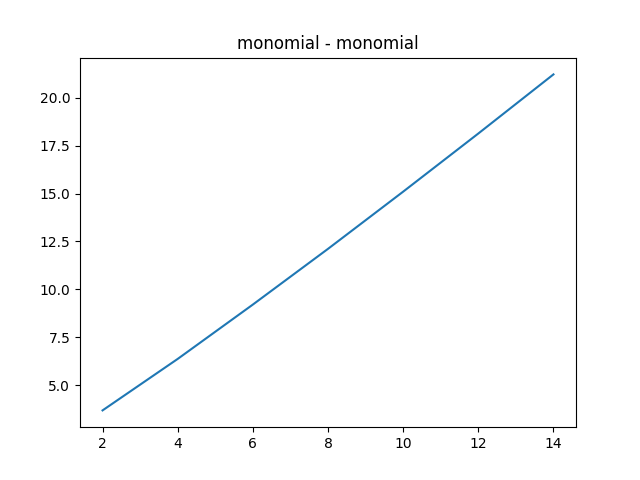
\includegraphics[width=\textwidth]{imgs/monomial_monomial.png}
         \caption[Monomial polynomial with monomial moment matrix]%
         {\small monomial polynomial with monomial moment matrix}% 

     \end{subfigure}
     \hfill
     \begin{subfigure}[b]{0.475\textwidth}  
         \centering 
         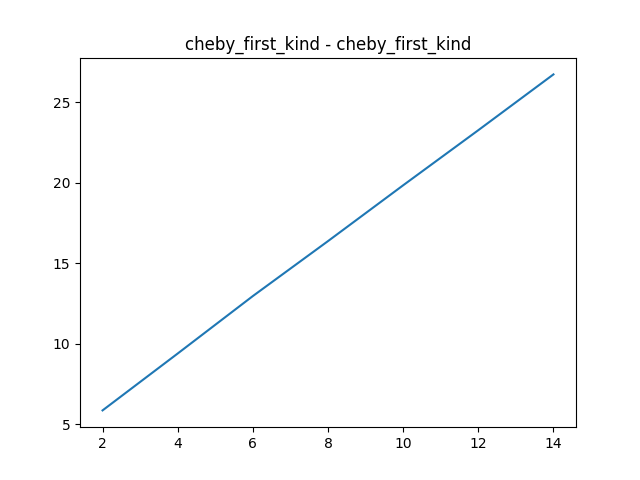
\includegraphics[width=\textwidth]{imgs/cheby_first_kind_cheby_first_kind.png}
         \caption[ChebyShev first kind polynomial with ChebyShev first kind moment matrix]%
         {\small ChebyShev first kind polynomial with ChebyShev first kind moment matrix}% 
 
     \end{subfigure}
     \vskip\baselineskip
     \begin{subfigure}[b]{0.475\textwidth}   
         \centering 
         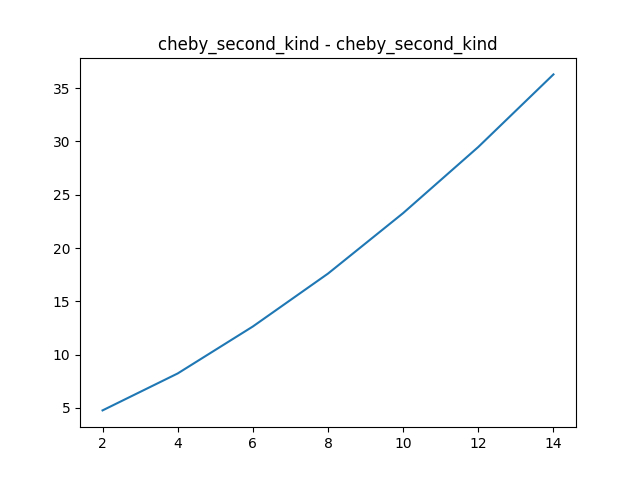
\includegraphics[width=\textwidth]{imgs/cheby_second_kind_cheby_second_kind.png}
         \caption[ChebyShev second kind polynomial with ChebyShev second kind moment matrix]%
         {\small ChebyShev second kind polynomial with ChebyShev second kind moment matrix}% 

     \end{subfigure}
     \hfill
     \begin{subfigure}[b]{0.475\textwidth}   
         \centering 
         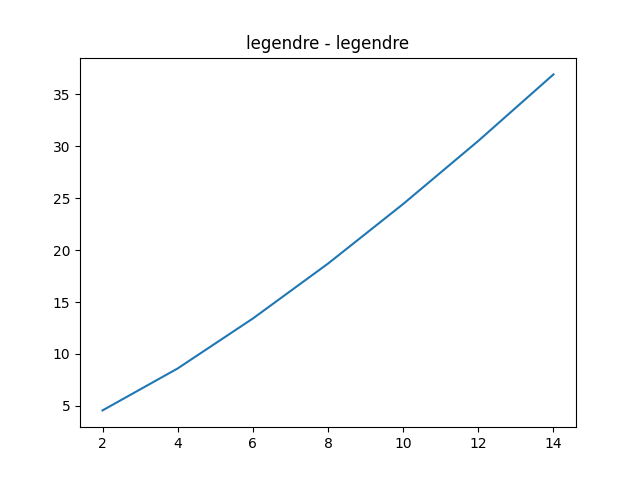
\includegraphics[width=\textwidth]{imgs/legendre_legendre.png}
         \caption[Legendre polynomial with legendre moment matrix]%
         {\small Legendre polynomial with legendre moment matrix}% 
     \end{subfigure}
     \caption[ Condition number of the coefficient moment matrix for same basis]%
     {\small Condition number of the coefficient moment matrix for same basis (univ)}% 
 \end{figure*}

Another phenomenon that we observe is that the monomial polynomial base do not work well
with orthogonal polynomial bases. When using monomial to serve as the polynomial basis of Moment Matrix
and using orthogonal polynomial basis to express the original polynomial,
or the other way around, 
the condition number of the coefficient moment matrix tends 
to blow up with the increasing of the degree of the polynomials.

\begin{figure*}[h]
     \centering
     \begin{subfigure}[b]{0.475\textwidth}
         \centering
         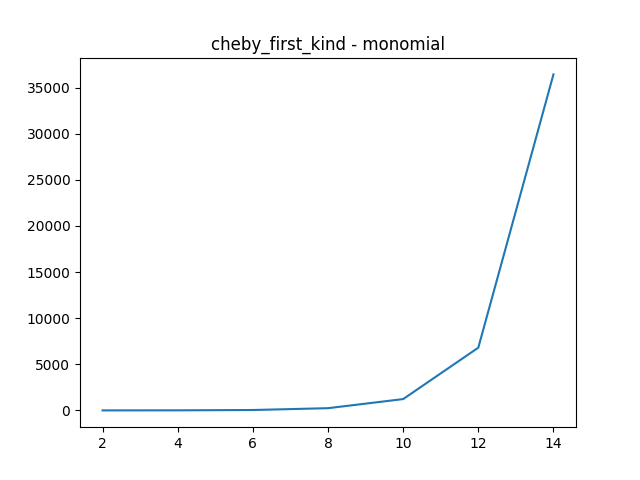
\includegraphics[width=\textwidth]{imgs/cheby_first_kind_monomial.png}
         \caption[ChebyShev First Kind polynomial with monomial moment matrix]%
         {\small ChebyShev first kind polynomial with monomial moment matrix}% 

     \end{subfigure}
     \hfill
     \begin{subfigure}[b]{0.475\textwidth}  
         \centering 
         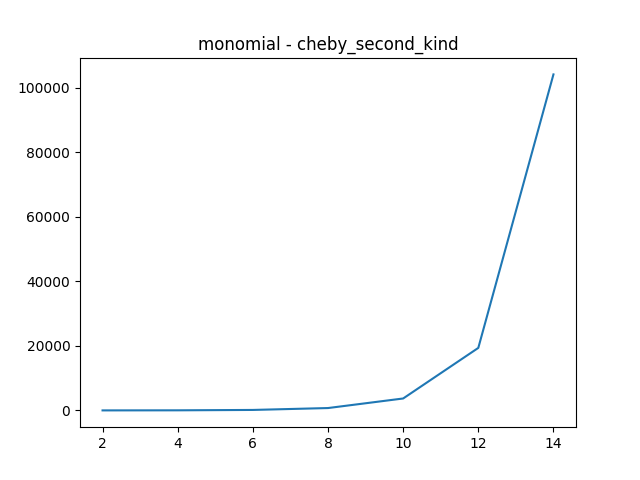
\includegraphics[width=\textwidth]{imgs/monomial_cheby_second_kind.png}
         \caption[monomial polynomial with ChebyShev second Kind moment matrix]%
         {\small monomial polynomial with ChebyShev second Kind moment matrix}% 
 
     \end{subfigure}
     \vskip\baselineskip
     \begin{subfigure}[b]{0.475\textwidth}   
         \centering 
         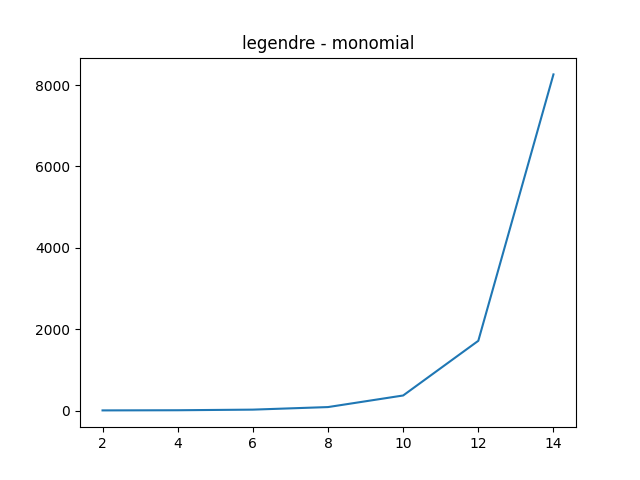
\includegraphics[width=\textwidth]{imgs/legendre_monomial.png}
         \caption[Legendre polynomial with monomial moment matrix]%
         {\small Legendre polynomial with monomial moment matrix}% 

     \end{subfigure}
     \hfill
     \begin{subfigure}[b]{0.475\textwidth}   
         \centering 
         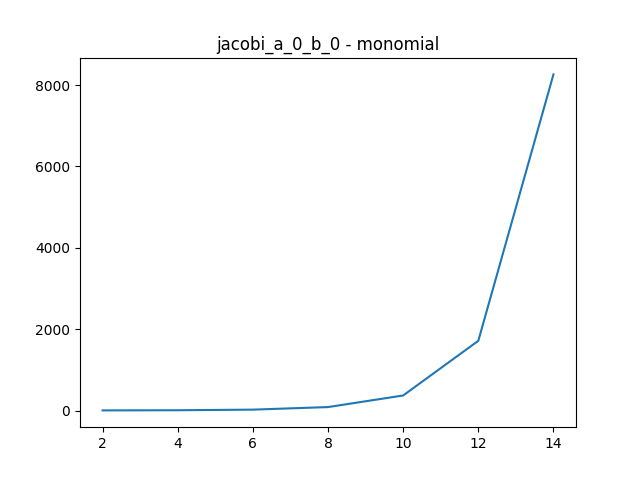
\includegraphics[width=\textwidth]{imgs/jacobi_a_0_b_0_monomial.png}
         \caption[Jacobi polynomial with monomial moment matrix]%
         {\small Jacobi polynomial with monomial moment matrix}% 
     \end{subfigure}
     \caption[ Monomial with Orthogonal Polynomials ]%
     {\small Monomial with Orthogonal Polynomials (univ)}% 
 \end{figure*}

On the other hand, the orthogonal polynomials tend to work very well when they are between each other.
We can see the scale of the condition number for is dramatically smaller than the condition numbers with monomial involved. 

 \begin{figure*}[h]
     \centering
     \begin{subfigure}[b]{0.475\textwidth}
         \centering
         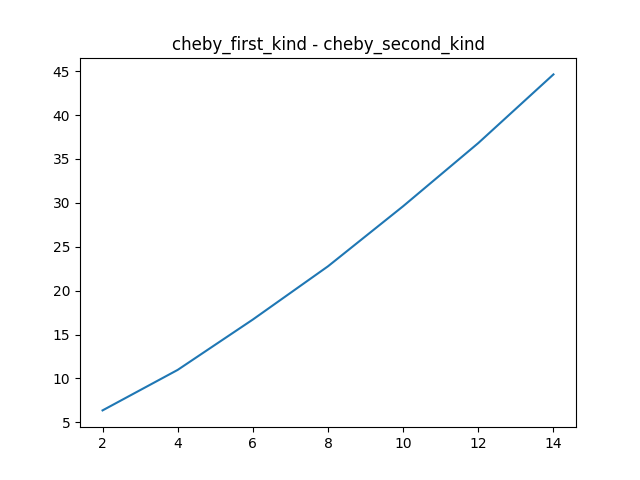
\includegraphics[width=\textwidth]{imgs/cheby_first_kind_cheby_second_kind.png}
         \caption[ChebyShev First Kind polynomial with monomial moment matrix]%
         {\small ChebyShev first kind polynomial with ChebyShev second kind moment matrix}% 

     \end{subfigure}
     \hfill
     \begin{subfigure}[b]{0.475\textwidth}  
         \centering 
         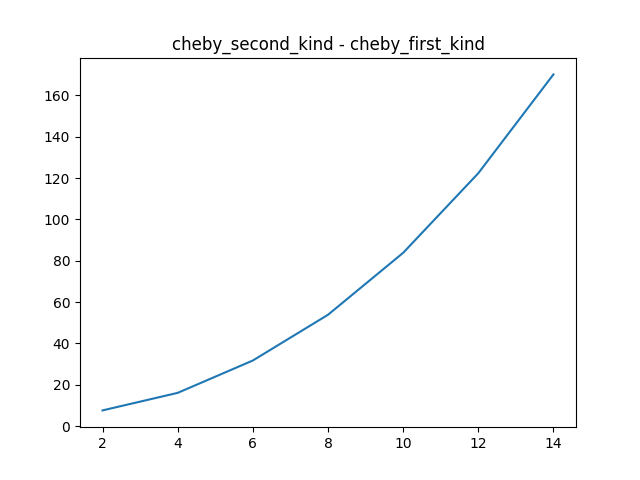
\includegraphics[width=\textwidth]{imgs/cheby_second_kind_cheby_first_kind.png}
         \caption[ChebyShev second kind polynomial with ChebyShev first kind moment matrix]%
         {\small ChebyShev second kind polynomial with ChebyShev first kind moment matrix}% 
 
     \end{subfigure}
     \vskip\baselineskip
     \begin{subfigure}[b]{0.475\textwidth}   
         \centering 
         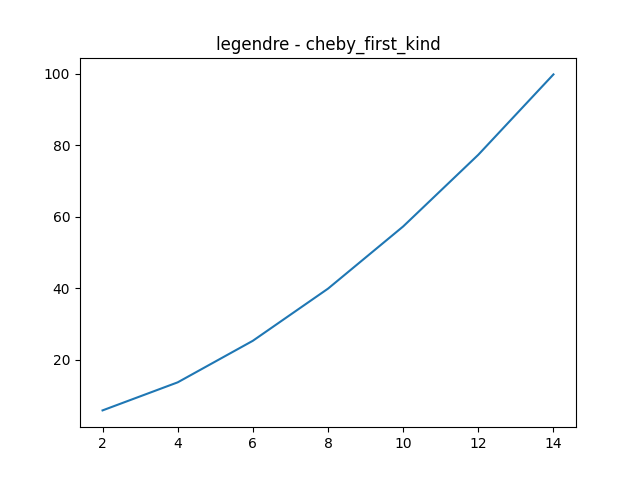
\includegraphics[width=\textwidth]{imgs/legendre_cheby_first_kind.png}
         \caption[Legendre polynomial with ChebyShev first kind moment matrix]%
         {\small Legendre polynomial with ChebyShev first kind moment matrix}% 

     \end{subfigure}
     \hfill
     \begin{subfigure}[b]{0.475\textwidth}   
         \centering 
         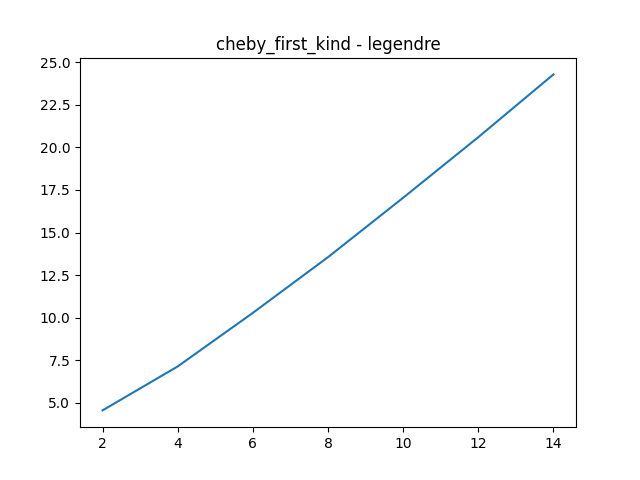
\includegraphics[width=\textwidth]{imgs/cheby_first_kind_legendre.png}
         \caption[Chebyshev first kind polynomial with Legendre moment matrix]%
         {\small Chebyshev first kind polynomial with Legendre moment matrix}% 
     \end{subfigure}
     \caption[ Monomial with Orthogonal Polynomials ]%
     {\small Monomial with Orthogonal Polynomials (univ)}% 
 \end{figure*}

 \newpage
Here, we summarize the results in a table of the 4 polynomials we are experimented with when the degree of the polynomial is 14. 
We left out the Jacobi polynomial, because Chebyshev polynomials and Legendre polynomials are special cases of it.
\begin{table*}[h]
     \small
     \begin{tabular}{|l||*{4}{c|}}\hline

          \backslashbox[50mm]{Polynomial Basis}{Moment Matrix Basis}
          &\makebox[6em]{Monomial}&\makebox[6em]{Chebyshev 1st}
          &\makebox[6em]{Chebyshev 2nd}&\makebox[6em]{Legendre}\\\hline\hline
          Monomial & 2.122801e+01 & 8.866559e+04 & 1.040619e+05 & 4.401169e+04	\\\hline
          Chebyshev 1st & 3.643853e+04 & 2.673064e+01 & 4.463266e+01 & 2.428417e+01\\\hline
          Chebyshev 2nd &5.248902e+04 & 1.701201e+02 & 3.629213e+01 & 7.221286e+01\\\hline
          Legendre & 8.260979e+03	& 9.981569e+01 & 6.871414e+01 & 3.691980e+01\\\hline
          
          \end{tabular}
          \caption{\label{tab:table-name}condition num of coefficient moment matrix with degree 14 (univ).}
\end{table*}
\newpage
\subsection{Bivariate Polynomials}
We performed the same experiments for the bivariate cases. We stopped the experiments when the degree of the polynomial reaches 8, 
which is smaller than 14, what we did for the univariate case, due to the computational cost. 
We observe similar phenomenon as in univariate case.

Just like in the univariate case, in general, the condition number is smaller when the basis of the polynomials and the basis of the moment matrix is the same. 
The monomial still have the smallest condition number, and Chebyshev first kind is outperforming other orthogonal basis by a small margin. 

\begin{figure*}[h]
     \centering
     \begin{subfigure}[b]{0.475\textwidth}
         \centering
         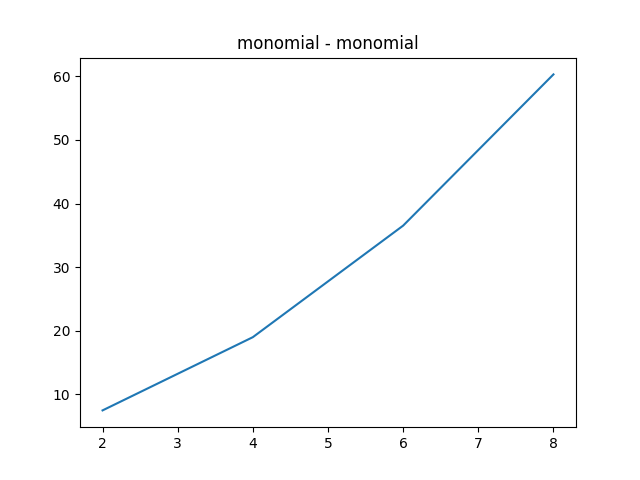
\includegraphics[width=\textwidth]{imgs_biv/monomial_monomial.png}
         \caption[Monomial polynomial with monomial moment matrix]%
         {\small monomial polynomial with monomial moment matrix}% 

     \end{subfigure}
     \hfill
     \begin{subfigure}[b]{0.475\textwidth}  
         \centering 
         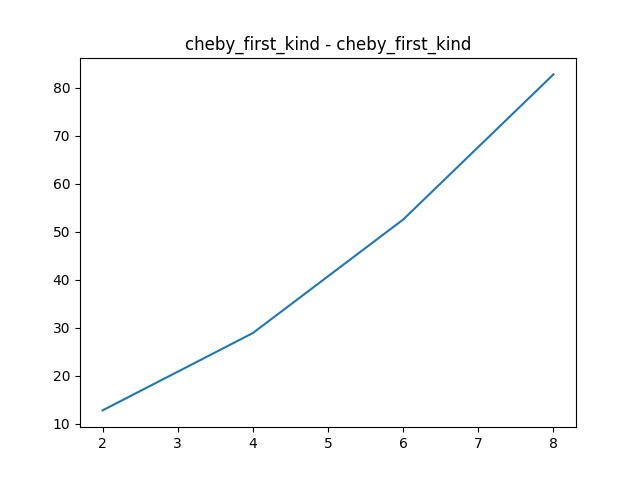
\includegraphics[width=\textwidth]{imgs_biv/cheby_first_kind_cheby_first_kind.png}
         \caption[ChebyShev first kind polynomial with ChebyShev first kind moment matrix]%
         {\small ChebyShev first kind polynomial with ChebyShev first kind moment matrix}% 
 
     \end{subfigure}
     \vskip\baselineskip
     \begin{subfigure}[b]{0.475\textwidth}   
         \centering 
         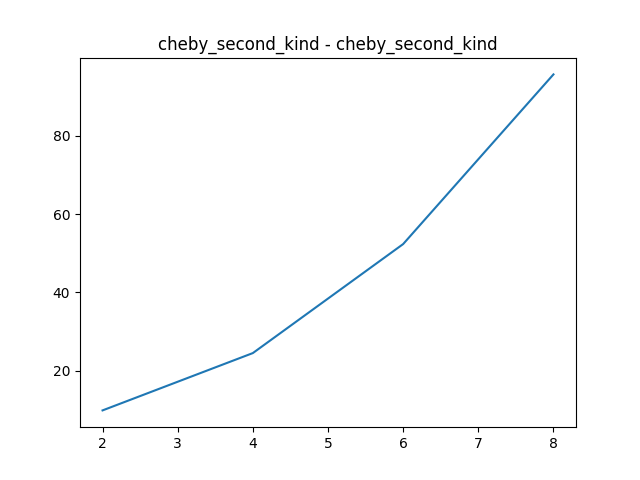
\includegraphics[width=\textwidth]{imgs_biv/cheby_second_kind_cheby_second_kind.png}
         \caption[ChebyShev second kind polynomial with ChebyShev second kind moment matrix]%
         {\small ChebyShev second kind polynomial with ChebyShev second kind moment matrix}% 

     \end{subfigure}
     \hfill
     \begin{subfigure}[b]{0.475\textwidth}   
         \centering 
         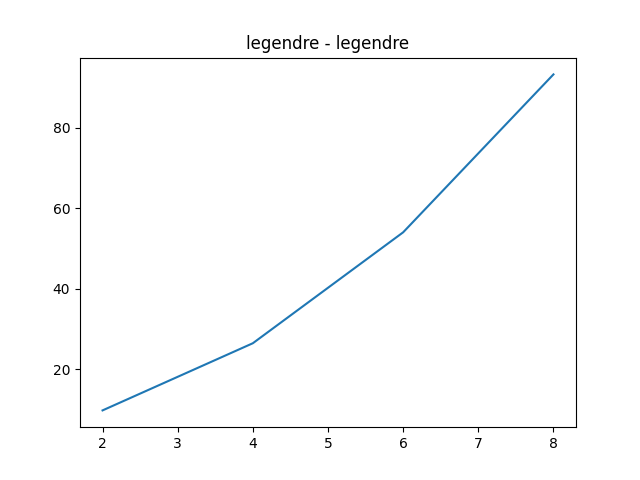
\includegraphics[width=\textwidth]{imgs_biv/legendre_legendre.png}
         \caption[Legendre polynomial with legendre moment matrix]%
         {\small Legendre polynomial with legendre moment matrix}% 
     \end{subfigure}
     \caption[ Condition number of the coefficient moment matrix for same basis]%
     {\small condition num of the coefficient moment matrix for same basis (biv)}% 
 \end{figure*}

When we have a combination of monomials and orthogonal polynomials, the condition number again grow very fast as
the degree of the polynomial increase. 

\begin{figure*}[h]
     \centering
     \begin{subfigure}[b]{0.475\textwidth}
         \centering
         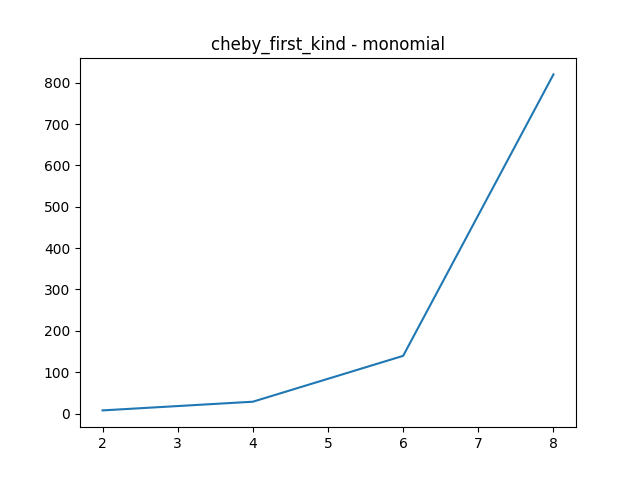
\includegraphics[width=\textwidth]{imgs_biv/cheby_first_kind_monomial.png}
         \caption[ChebyShev First Kind polynomial with monomial moment matrix]%
         {\small ChebyShev first kind polynomial with monomial moment matrix}% 

     \end{subfigure}
     \hfill
     \begin{subfigure}[b]{0.475\textwidth}  
         \centering 
         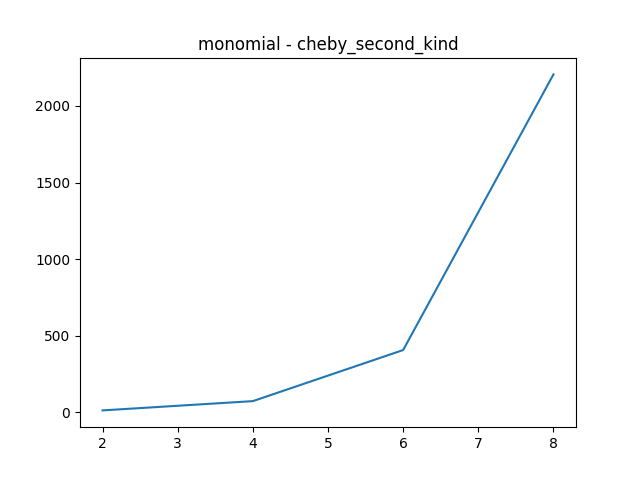
\includegraphics[width=\textwidth]{imgs_biv/monomial_cheby_second_kind.png}
         \caption[monomial polynomial with ChebyShev second Kind moment matrix]%
         {\small monomial polynomial with ChebyShev second Kind moment matrix}% 
 
     \end{subfigure}
     \vskip\baselineskip
     \begin{subfigure}[b]{0.475\textwidth}   
         \centering 
         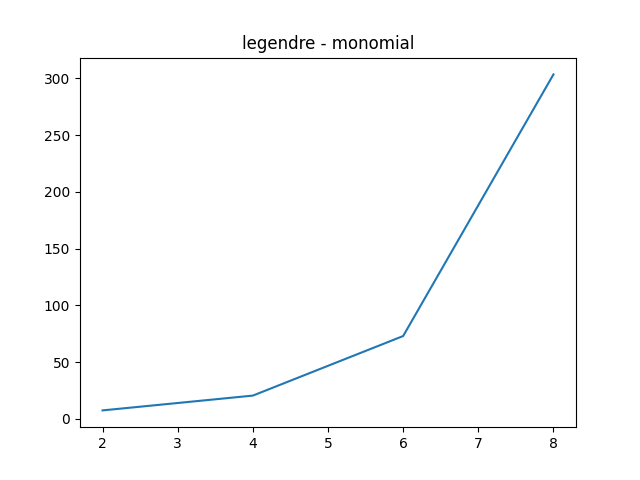
\includegraphics[width=\textwidth]{imgs_biv/legendre_monomial.png}
         \caption[Legendre polynomial with monomial moment matrix]%
         {\small Legendre polynomial with monomial moment matrix}% 

     \end{subfigure}
     \hfill
     \begin{subfigure}[b]{0.475\textwidth}   
         \centering 
         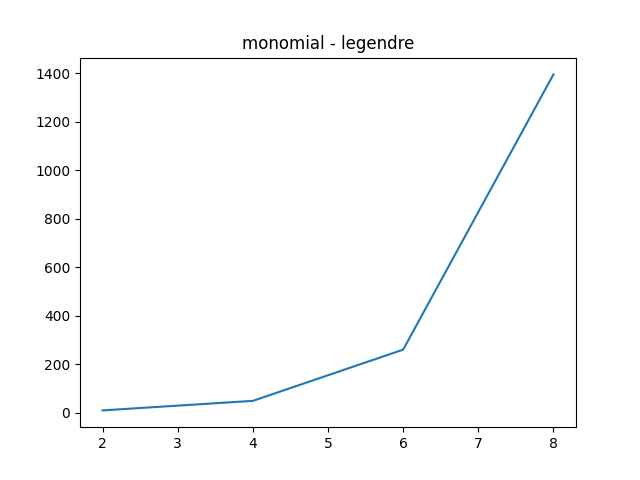
\includegraphics[width=\textwidth]{imgs_biv/monomial_legendre.png}
         \caption[Jacobi polynomial with monomial moment matrix]%
         {\small Jacobi polynomial with monomial moment matrix}% 
     \end{subfigure}
     \caption[ Monomial with Orthogonal Polynomials ]%
     {\small Monomial with Orthogonal Polynomials (biv)}% 
 \end{figure*}
\newpage
 When we are comingling orthogonal polynomials, the behavior of the system is more stable. 
 However, when we have Chebyshve first kind as the basis for the give polynomial
 and Legendre polynomial for the basis of the coefficient moment matrix, the condition number is 
 actually lower comparing to we use both Chebyshev first kind or both Legendre basis.

 \begin{figure*}[h]
     \centering
     \begin{subfigure}[b]{0.475\textwidth}
         \centering
         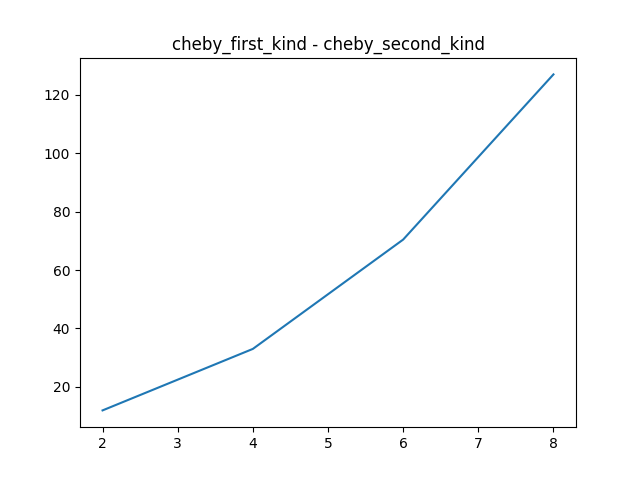
\includegraphics[width=\textwidth]{imgs_biv/cheby_first_kind_cheby_second_kind.png}
         \caption[ChebyShev First Kind polynomial with monomial moment matrix]%
         {\small ChebyShev first kind polynomial with ChebyShev second kind moment matrix}% 

     \end{subfigure}
     \hfill
     \begin{subfigure}[b]{0.475\textwidth}  
         \centering 
         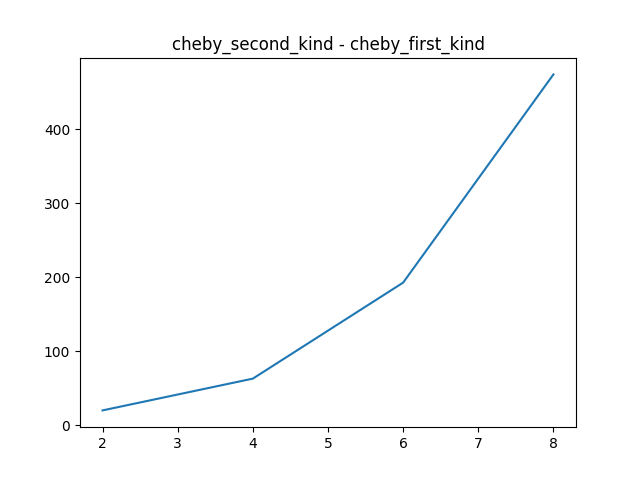
\includegraphics[width=\textwidth]{imgs_biv/cheby_second_kind_cheby_first_kind.png}
         \caption[ChebyShev second kind polynomial with ChebyShev first kind moment matrix]%
         {\small ChebyShev second kind polynomial with ChebyShev first kind moment matrix}% 
 
     \end{subfigure}
     \vskip\baselineskip
     \begin{subfigure}[b]{0.475\textwidth}   
         \centering 
         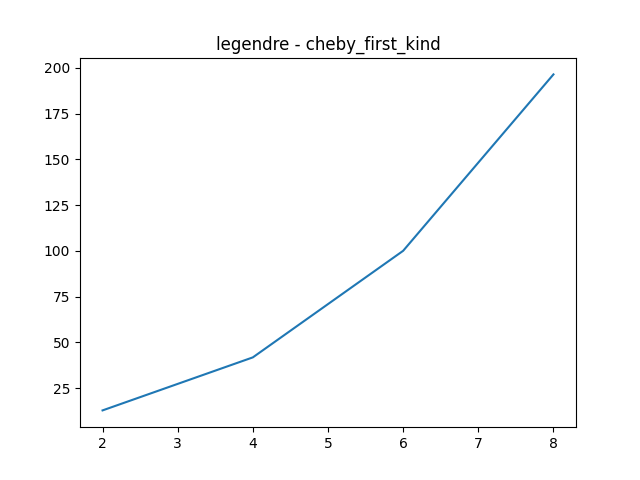
\includegraphics[width=\textwidth]{imgs_biv/legendre_cheby_first_kind.png}
         \caption[Legendre polynomial with ChebyShev first kind moment matrix]%
         {\small Legendre polynomial with ChebyShev first kind moment matrix}% 

     \end{subfigure}
     \hfill
     \begin{subfigure}[b]{0.475\textwidth}   
         \centering 
         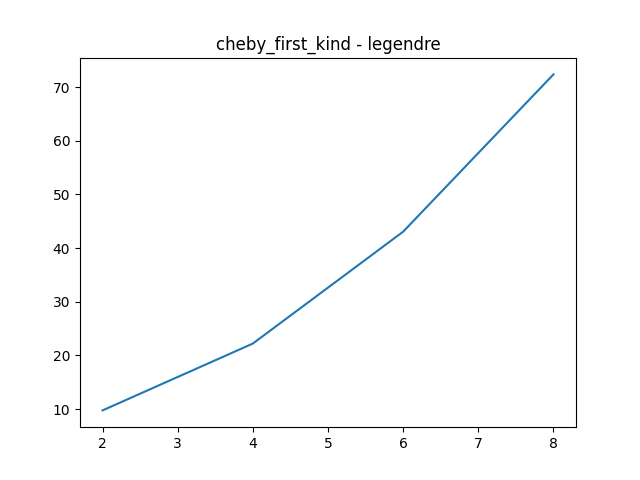
\includegraphics[width=\textwidth]{imgs_biv/cheby_first_kind_legendre.png}
         \caption[Chebyshev first kind polynomial with Legendre moment matrix]%
         {\small Chebyshev first kind polynomial with Legendre moment matrix}% 
     \end{subfigure}
     \caption[ Monomial with Orthogonal Polynomials ]%
     {\small Monomial with Orthogonal Polynomials (biv)}% 
 \end{figure*}
 \newpage
 Here, we do two tables to summarize the condition number of the combinations of the 4 basis that we tested on
 in both univariate case and bivariate case. When comparing the two tables, we can see that the condition number is 
 significantly larger than the univariate case. 
 \newpage
 \begin{table*}[h]
     \small
     \begin{tabular}{|l||*{4}{c|}}\hline

          \backslashbox[50mm]{Polynomial Basis}{Moment Matrix Basis}
          &\makebox[6em]{Monomial}&\makebox[6em]{Chebyshev 1st}
          &\makebox[6em]{Chebyshev 2nd}&\makebox[6em]{Legendre}\\\hline\hline
          Monomial & 1.2114041e+01 & 9.2931794e+02 & 7.3426803e+02 & 3.4094072e+02	\\\hline
          Chebyshev 1st & 2.4395198e+02 & 1.6377406e+01 & 2.2771550e+01 & 1.3558274e+01 \\\hline
          Chebyshev 2nd & 4.4894498e+02 & 5.3861887e+01 & 1.7604737e+01 & 2.9399442e+01 \\\hline
          Legendre & 8.5482089e+01	& 3.9905724e+01 & 3.2969591e+01 & 1.8699677e+01 \\\hline
          
          \end{tabular}
          \caption{\label{tab:table-name}condition num of coefficient moment matrix with degree 8 (univ).}
\end{table*}

 \begin{table*}[h]
     \small
     \begin{tabular}{|l||*{4}{c|}}\hline

          \backslashbox[50mm]{Polynomial Basis}{Moment Matrix Basis}
          &\makebox[6em]{Monomial}&\makebox[6em]{Chebyshev 1st}
          &\makebox[6em]{Chebyshev 2nd}&\makebox[6em]{Legendre}\\\hline\hline
          Monomial & 6.0303522e+01 & 3.8821664e+03 & 2.2060581e+03 & 1.3954908e+03	\\\hline
          Chebyshev 1st & 8.2003242e+02 & 8.2741589e+01 & 1.2690227e+02 & 7.2356027e+01\\\hline
          Chebyshev 2nd & 1.3583584e+03 & 4.7372727e+02 & 9.5693596e+01 & 2.0181265e+02\\\hline
          Legendre & 3.0351806e+02	& 1.9649165e+02 & 1.4316038e+02 & 9.3276473e+01 \\\hline
          
          \end{tabular}
          \caption{\label{tab:table-name}condition num of coefficient moment matrix with degree 8 (biv).}
\end{table*}
\newpage
%\begin{figure}

%\end{figure}

\newpage


\section{Discussion and Outlook}
\label{Sec:Dis and Outlook}

In this section, we state the observations that we made when generating the numerical results that we presented in the above section,
and we also state some open problems that related to our findings for potential future efforts. 

To begin, we observe that using monomials basis as both basis for input polynomials and basis for the coefficient moment matrix 
tends to be a good choice, since it constantly have very low condition number. 
Therefore, the linear system that generated by COC is more robust when the input data is interpolated by random noises. 
Moreover, when performing the experiments, the moment matrix with monomial basis has faster running time, 
where we measure running time by computer time rather than in complexity theory terms. 
As a result, deceivingly, one tends to conclude that we should just choose monomial bases for both input polynomial and the coefficient moment matrix.
However, this is not true. 
In fact, monomial basis has disadvantages in stability and running time. 

In terms of the stability, in many cases
the basis that the input polynomial is using is determined by the applications rather than by us when performing optimization.
From we can see in the above section, if the input polynomials are expressed in orthogonal basis, then choosing monomial 
polynomials as the basis if the coefficient moment matrix would horribly destroy the stability of the system as the condition number of the linear system blow up very quickly. 
One might argue that we can simply perform a change of basis to convert orthogonal basis to monomials. However,
this will also introduce the same level, if not more, of the changes to the condition numbers, because we would need to
consider the condition number of the change of a basis matrix as well. 
Hence, in that case we need to choose the suitable polynomial basis for our coefficient moment matrix that best serves the applications. 

In terms of the running time, the reason that monomial basis have faster computer time is because when using orthogonal polynomials as the basis of the coefficients moment matrix, 
we need to evaluate an integral that is needed for the orthogonal basis to extract the coefficients. 
However, in applications, this is more or less is an overhead work that one shall perform before executing optimizations. 
The reason is in applications, the number of variate and degree of the polynomials involved are pre-determined. 
Therefore, one could just calculate the needed integral for each basis beforehand. 
Hence, when performing the optimizations, 
all one need to do is exploiting the linearity of the integrations to extract the coefficients that are needed. 
Because of that, each step in the optimization process would only require constant time multiplication to 
obtain the coefficients, rather than performing $O(mk + nd + l)$ coefficients extraction algorithm as indicated in \ref{alg:mcem}.

As a result, one should try to use orthogonal basis in the coefficient moment matrix when the application allows to and 
the stability of the linear system generated by the COC algoirthm is not too poor.

Another observation that we can easily make, which is also indicted in the previous section, 
is that when comingle monomial basis with orthogonal basis, the condition number of the linear system expload very fast. 
This is a question that we didn't find an immediate answer to it. 
One conjecture that we can make is because the orthogonal polynomials are all special cases of Jacobi polynomials,
they share similar structures in their bases. As a result, when performing the integration, the result is relatively stable. 
However, this might be a question that worth to take a closer look.
Maybe there are some structures that polynomial basis has that can be used to deduce the stability of the system, rather than using numerical experiments. 

Lastly, we would like to state, other than the canonical SOS certificate of the nonnegativity of polynomials, 
there are many other certificates that captures different intuitions or have different usages in applications. 
For example, \emph{sums of nonnegative circuit polynomials} (SOPN)\cite{Iliman2016}, 
a recently introduced certificate of nonnegativity, is more applicable in constraint polynomial optimizations \cite{wang2021nonnegative},
and can be used to substitute (SOS) for optimization problems over hypercube, on which (SOS) has worse performance comparing to other algorithms \cite{dressler2018optimization}. 
Therefore, it would also be interesting to see whether different choices of polynomial basis can impact the stability of
the system generated when using other certificates to try to determine whether a polynomial is nonnegative or not.




%\section*{Acknowledgements}
%We thank the anonymous referees for their helpful comments.


\newpage
\bibliographystyle{amsalpha}
\bibliography{main}

\end{document}
